\chapter{Evaluating the Robustness of the \emph{EvoTSC} Model}
\label{chap:param}

In this chapter, I explore the robustness of the characteristics of evolving populations to variations in the parameters of the \emph{EvoTSC} model.
To this aim, I present several sets of additional evolutionary simulations.
In these simulations, I first measure whether populations are able to evolve differentiated gene expression patterns as a response to different environments in the model variants.
I then compare the speed of evolution of these populations with the main runs presented in Chapter~\ref{chap:ploscb}.
I first explore the sensitivity of the model to the genome-level parameters (see Table~\ref{tab:param:params} below): the maximum interaction distance for the transcription-supercoiling coupling, the mean intergenic distance, and the strength of the environment-caused shift in background supercoiling.
I then investigate simulating a higher number of genes on the genome.
Finally, I discuss the evolutionary effect of allowing intergenic distances to mutate, by introducing indels in intergenic sections as a new mutational operator in the model.
The data from this experiment is available online on the \href{https://doi.org/10.5281/zenodo.7304906}{Zenodo} platform.

\begin{table}[H]
\begin{center}
\begin{tabular}{l c r r}
\toprule
\textbf{Parameter} & \textbf{Symbol} & \textbf{Value} & \textbf{\# of Replicates} \\
\midrule
Interaction distance & $d_{max}$ & \textbf{5 kb} & \textbf{30}\\
(Section~\ref{sec:param:inter25k}) & & 25 kb & 15\\
\midrule
& & 10 bp& 15\\
Mean intergenic size & $d_{mean}$ & \textbf{125 bp} & \textbf{30} \\
(Section~\ref{sec:param:mean-intergene})& & 1,000 bp & 15\\
& & 10,000 bp & 15 \\
\midrule
& & 0.0001 & 15\\
Environment supercoiling shift & $\delta\sigma_{A/B}$ & 0.001 & 15\\
(Section~\ref{sec:param:sigma-env})& & \textbf{0.01} & \textbf{30}\\
%\midrule
%Number of genes & $n$ & \textbf{60} & \textbf{30} \\
%(Section~\ref{sec:param:300-genes})& & 30 & 15 \\
\bottomrule
\end{tabular}
\end{center}
\caption[Table of parameter values explored in additional \emph{EvoTSC} simulations]{Table of the parameters and associated values explored in additional experiments (separated by horizontal lines).
For each experiment, the row in bold font corresponds to the parameter values used in the main run described in Chapter~\ref{chap:ploscb}, and is shown for reference.}
\label{tab:param:params}
\end{table}

\section{Interaction Distance}
\label{sec:param:inter25k}

The size of the topological domains of bacterial genomes, inside which DNA supercoils can freely propagate, has historically been estimated to be on the order of a few thousand base pairs~\citep{elhanafi2000,postow2004,kouzine2013}.
Recent work has however suggested that the size of transcription-generated twin domains could be much larger than this, and reach up to 25 kb on either side of the transcribed gene~\citep{visser2022}.
As the size of the topological domains sets a limit to the number of genes that can interact through the transcription-supercoiling coupling, it is likely to play an important role in the structure of the supercoiling-mediated gene regulatory networks.
By increasing the number of genes a given gene is coupled with, a larger interaction distance could make genomic inversions more deleterious by making them disrupt a larger part of the regulatory networks at their boundaries, but it could also allow more robust regulatory networks to evolve through a higher connectivity.
In this section, I present simulations run with an interaction distance of 25 kb, a five-fold increase from the value used in the main runs, in order to test these hypotheses.

\begin{figure}[H]
\centering
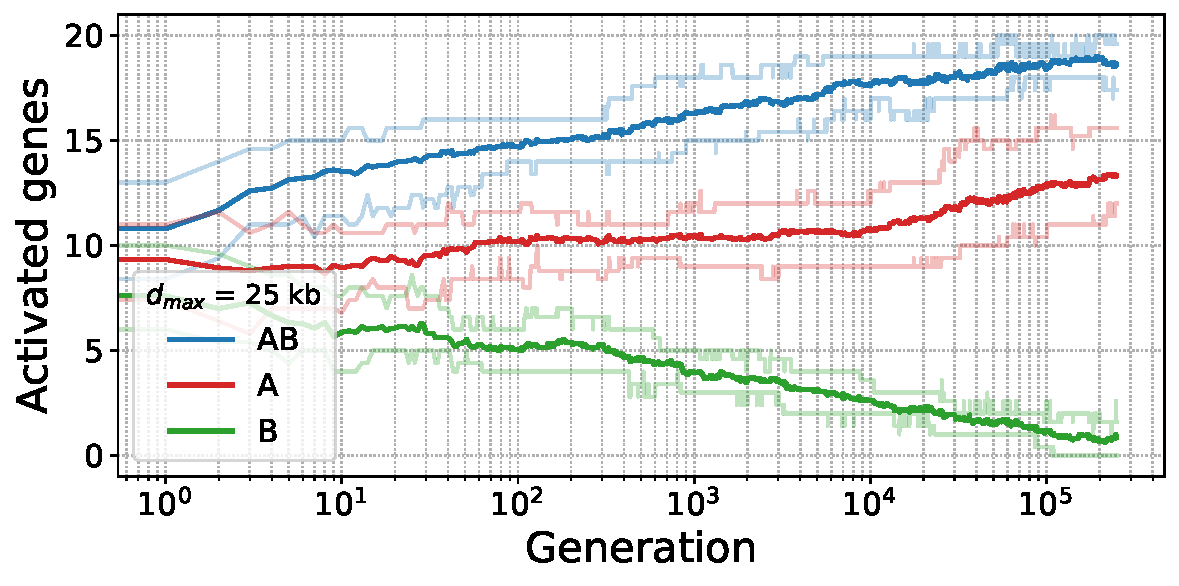
\includegraphics[width=0.495\textwidth]{param/interaction-25k/gene_activity_env_A.pdf}
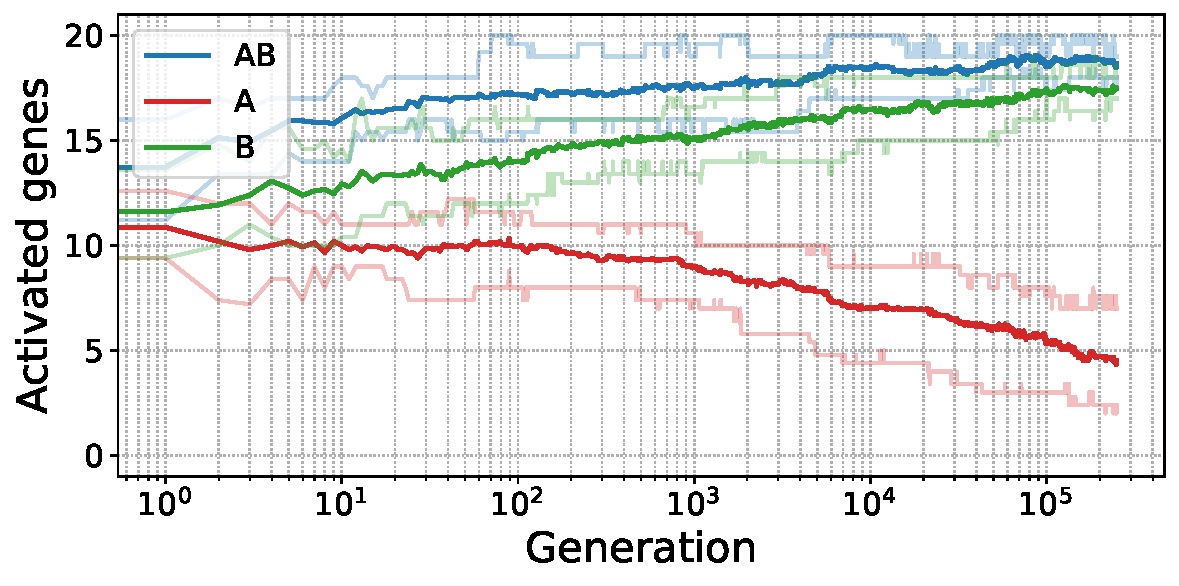
\includegraphics[width=0.495\textwidth]{param/interaction-25k/gene_activity_env_B.pdf}
\caption[Evolution of the number of activated genes in each environment, with an interaction distance of 25 kb]{Evolution of the number of activated genes in environment A (left) and environment B (right), with an interaction distance of 25 kb.
Lighter lines represent the first and last decile of the data.}
\label{fig:param:inter25k-activ-by-env}
\end{figure}

Figure~\ref{fig:param:inter25k-activ-by-env} shows the evolution of the number of activated genes of each type in the simulations with the interaction distance of 25 kb, over 250,000 generations (to be compared to Figure~\ref{fig:ploscb:gene_activity_by_env} in Chapter~\ref{chap:ploscb}).
As in the main run, the number of activated genes of each type evolves towards their respective target.
Differentiated activation patterns can therefore still evolve even when the topological domains are 5 times larger.

\begin{figure}[H]
\centering
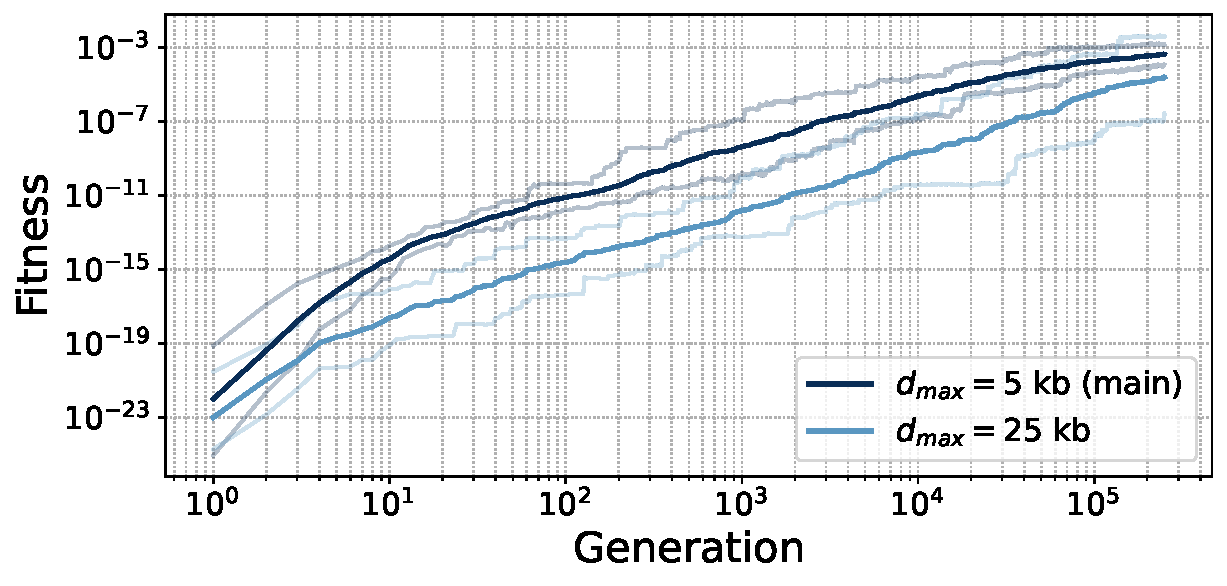
\includegraphics[width=0.8\textwidth]{param/interaction-25k/fitness_all_with_main.pdf}
\caption[Average fitness during evolution, with an interaction distance of 25 kb]{Average fitness during evolution with an interaction distance of 25 kb (light blue), and in the main run (dark blue).
Lighter lines represent the first and last decile of the data.}
\label{fig:param:inter25k-fitness}
\end{figure}

Figure~\ref{fig:param:inter25k-fitness} shows the evolution of the average fitness of the best individual in each replicate of the simulation with a larger interaction distance, compared with the evolution of fitness in the main run, over 250,000 generations.
While fitness is systematically lower throughout evolution with the larger interaction distance, it nonetheless follows a qualitatively similar curve, and keeps on increasing until the end of the runs, suggesting that it could eventually reach the same value as in the main run (presented in full in Figure~\ref{fig:ploscb:main_fitness}).

\begin{figure}[H]
\centering
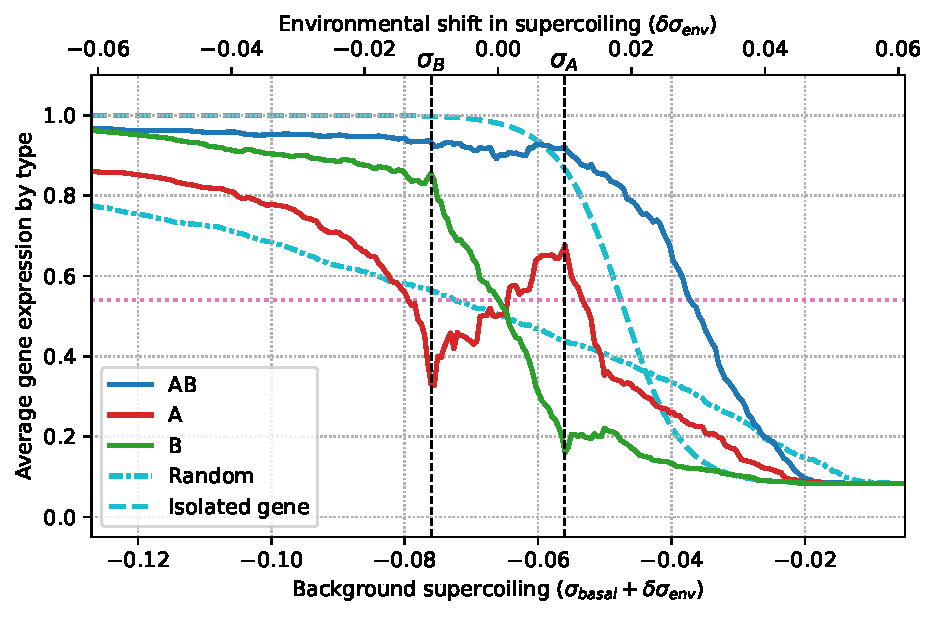
\includegraphics[width=0.9\textwidth]{param/interaction-25k/activity_sigmas_avg.pdf}
\caption[Average gene expression as a function of background supercoiling, with an interaction distance of 25 kb]{Average gene expression by type as a function of background supercoiling, with an interaction distance of 25 kb.
The dash-dotted line represents the average expression of genes on a random genome with an interaction distance of 25 kb.}
\label{fig:param:inter25k-activ-by-sigma}
\end{figure}

Figure~\ref{fig:param:inter25k-activ-by-sigma} shows the average gene expression by type of evolved individuals, as a function of the background supercoiling level.
As in the main run, \emph{A} genes display a relaxation-activated phenotype.
\emph{AB} and \emph{B} genes are relaxation-inhibited, but nonetheless display quite different behaviors than the (dash-dotted light blue) curve for genes on a random genome with the same parameters, which present a much flatter response curve to background supercoiling than with the default interaction distance of 5 kb (shown in Figure~\ref{fig:ploscb:activity-by-sigma}).

\begin{figure}[H]
\centering
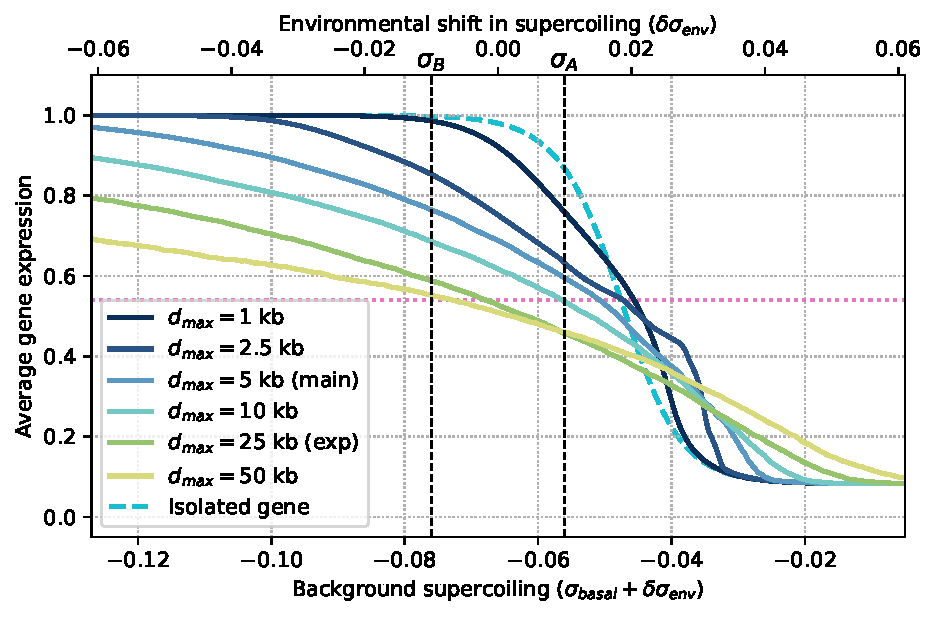
\includegraphics[width=0.9\textwidth]{param/interaction-25k/random_activ_per_sigma.pdf}
\caption[Average gene expression as a function of background supercoiling, with increasing interaction distances, in random genomes]{Average gene expression as a function of background supercoiling in random genomes with increasing interaction distances (full lines), and theoretical expression level of an isolated gene (dashed line).}
\label{fig:param:inter25k-random-activ-by-sigma}
\end{figure}

Comparing the effect of background supercoiling variation on the transcriptional activity of genes on random genomes with an interaction distance of 5 kb (Figure~\ref{fig:ploscb:activity-by-sigma}) or 25 kb (Figure~\ref{fig:param:inter25k-activ-by-sigma}) seems to indicate that a larger interaction distance buffers the effect of the background supercoiling on gene expression in the model.
In order to test this hypothesis, I measured the average gene expression as a function of background supercoiling in random genomes with maximum interaction distances ranging from 1 kb to 50 kb, with an average intergenic distance remaining constant at 125 bp.
For each interaction distance, I generated 100 genomes, and made each genome undergo 100 replication events to shuffle the genes on the genome via genomic inversions.
Figure~\ref{fig:param:inter25k-random-activ-by-sigma} shows the result of this experiment.
As the interaction distance increases, the response curve of genes to a changing background supercoiling level indeed becomes flatter and flatter, which can be interpreted as a buffering of the effect of the environmental perturbation on gene expression by the supercoiling-mediated interaction of a higher and higher number of genes.
Conversely, as the interaction distance gets closer to zero, the curve is closer and closer to that of an isolated, non-interacting gene.


\begin{figure}[H]
\centering
\begin{subfigure}[t]{0.495\textwidth}
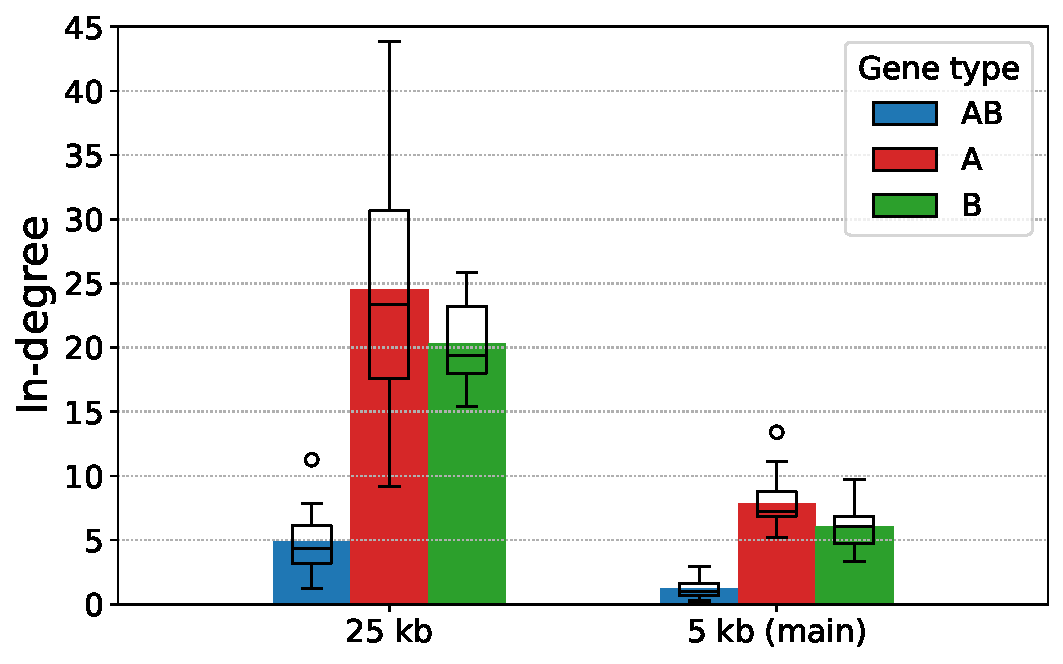
\includegraphics[width=\textwidth]{param/interaction-25k/effective_graph_combined_in_degree.pdf}
\end{subfigure}
\begin{subfigure}[t]{0.495\textwidth}
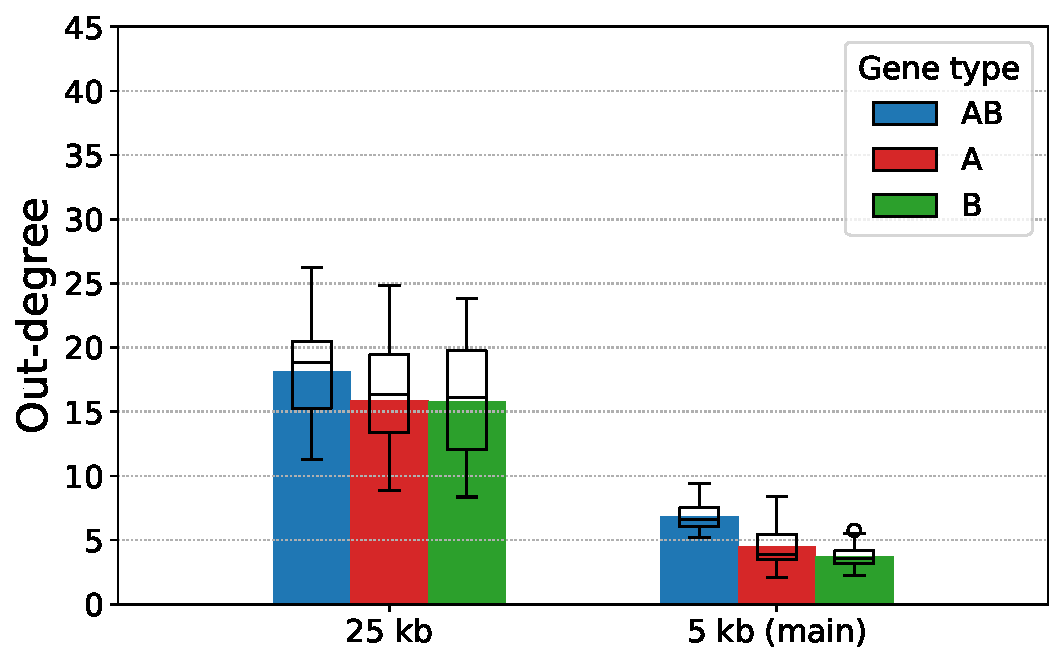
\includegraphics[width=\textwidth]{param/interaction-25k/effective_graph_combined_out_degree.pdf}
\end{subfigure}
\caption[Average in- and out-degree of effective interaction graph nodes, with an interaction distance of 25 kb]{Average out-degree (left) and in-degree (right) of the genes in the effective interaction graph, separated by gene type, for individuals with an interaction distance of 5 kb (main run) or 25 kb.}
\label{fig:param:inter25k-degree}
\end{figure}

Figure~\ref{fig:param:inter25k-degree} finally presents the average in- and out-degree of the genes in the effective interaction graph obtained with gene knockouts, compared to the same data from the main run.
As could be expected, the gene regulatory networks are much more connected with the larger interaction distance, but the behavior for each gene type remains qualitatively the same as in the main run.

Overall, the evolution of supercoiling-mediated gene regulatory networks that are able to show environment-specific activation patterns, and in particular relaxation-activated genes, therefore seems robust in our model to a larger interaction distance.
Even when the networks are more densely connected, buffering gene expression, the reorganization of the genome via genomic inversion allows for specific behaviors for each gene type.


\section{Mean Intergenic Size}
\label{sec:param:mean-intergene}

In the main run, I set the initial intergenic distance between every gene to 125 bp, or a gene density of 88\%, representing the average \emph{E. coli} intergenic distance~\citep{postow2004}.
Bacteria actually present a wider range of gene densities, from 51\% in \emph{Sodalis glossinidius}, a bacteria that is undergoing massive pseudogenization after recently adopting an endosymbiotic lifestyle~\citep{toh2006}, up to 95\% in \emph{Thermotoga maritima}, an extremophile bacteria living in heated marine sediment~\citep{nelson1999}.
Like the interaction distance, the mean intergenic distance plays a role in the connectivity of the gene regulatory networks that stem from the transcription-supercoiling coupling: when the mean intergenic distance is small, more genes can on average be affected by the transcription of any given gene.
Conversely, when the mean intergenic distance is large compared to the interaction distance, the emergence of regulatory subnetworks isolated from each other by large intergenic regions becomes possible.
In this section, I test the robustness of the results with regard to the range of gene densities found across living organisms.
I present simulations with mean intergenic distances increasing logarithmically from 10 bp (or a gene density of 99\%), comparable to the median intergenic distance of 3 bp found in \emph{Pelagibacter ubique}, a free-living marine bacteria~\citep{giovannoni2005}, up to 10 kb (or a gene density of 10\%), akin to the gene-scarce eukaryotic genomes~\citep{davilalopez2010}.

\begin{figure}[H]
\centering
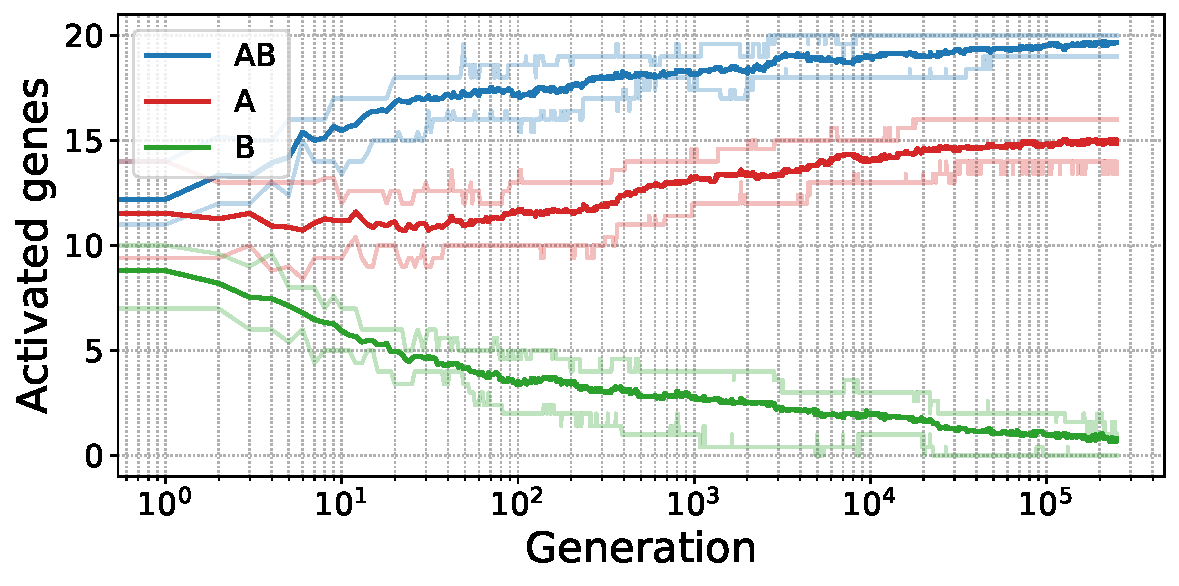
\includegraphics[width=0.495\textwidth]{param/mean-intergene/inter-0.01k/gene_activity_env_A.pdf}
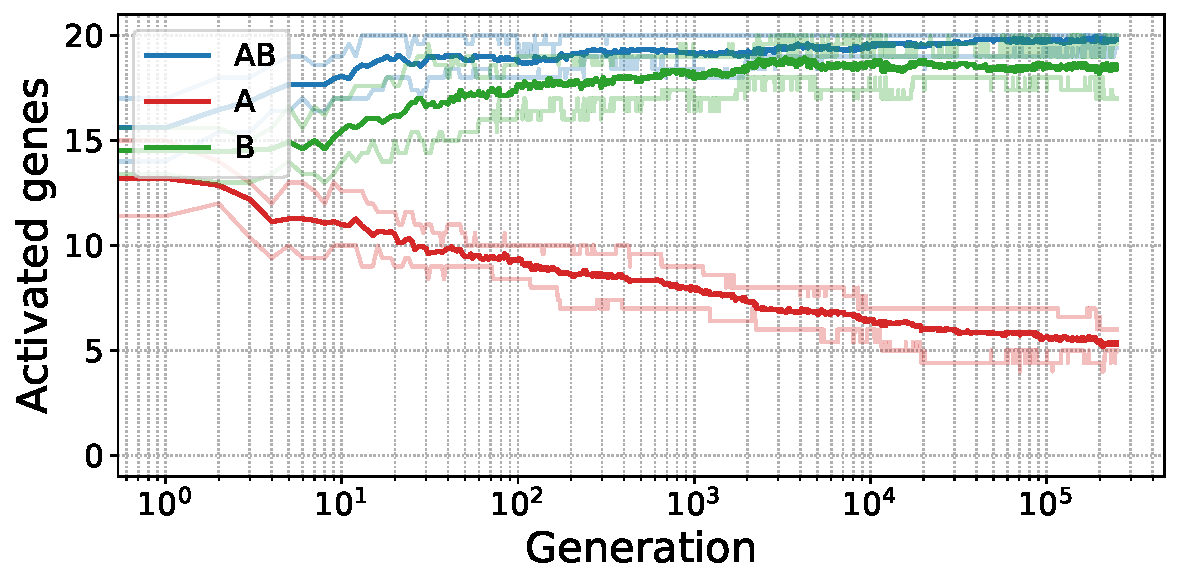
\includegraphics[width=0.495\textwidth]{param/mean-intergene/inter-0.01k/gene_activity_env_B.pdf}

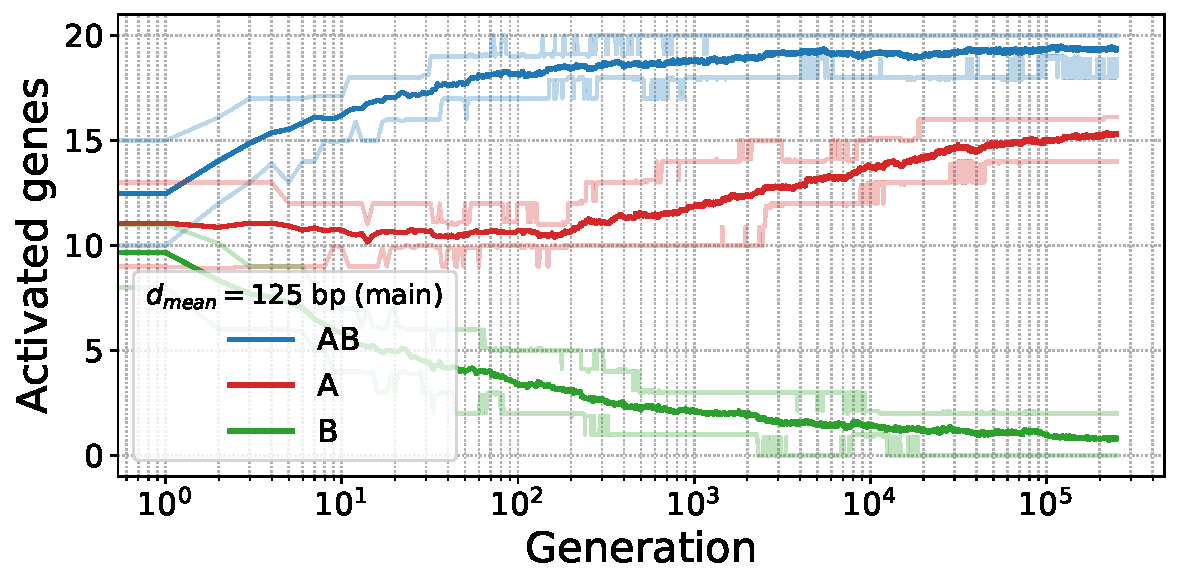
\includegraphics[width=0.495\textwidth]{param/mean-intergene/inter-0.125k/gene_activity_env_A.pdf}
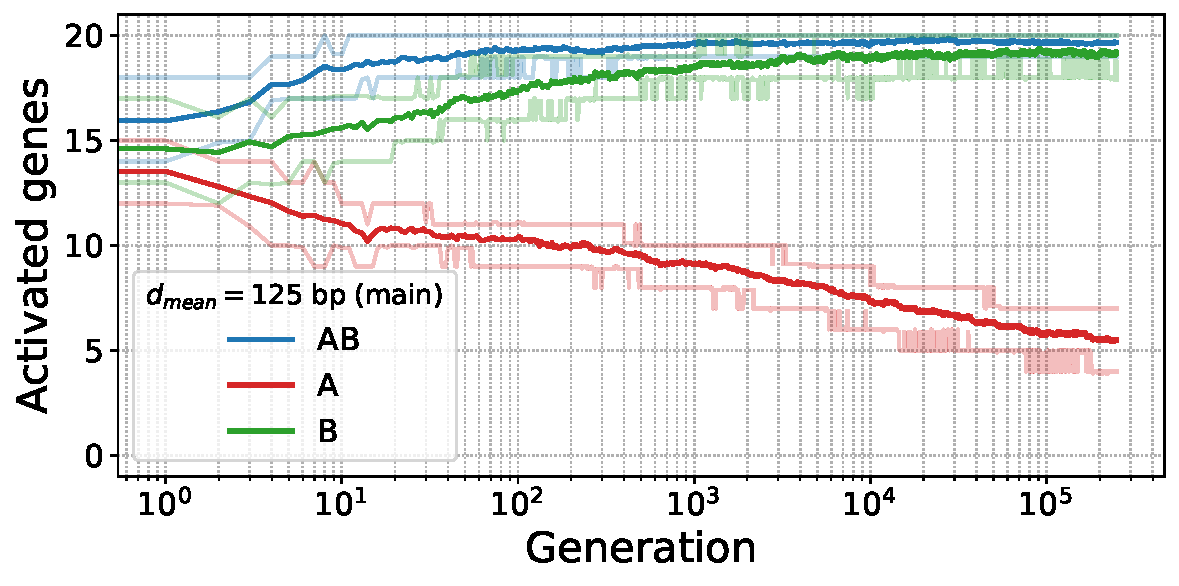
\includegraphics[width=0.495\textwidth]{param/mean-intergene/inter-0.125k/gene_activity_env_B.pdf}

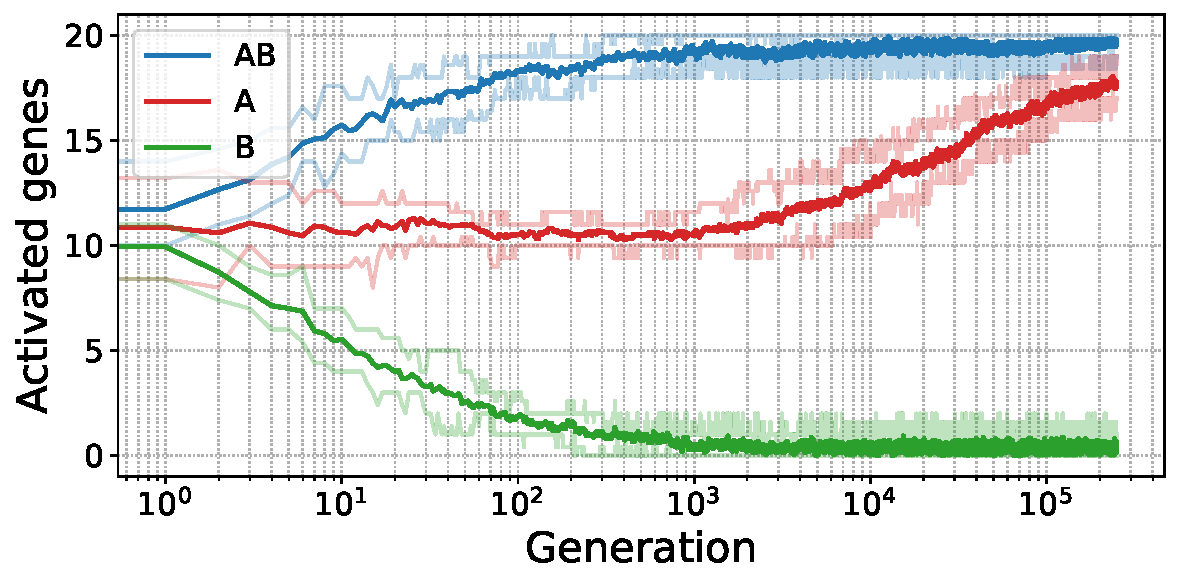
\includegraphics[width=0.495\textwidth]{param/mean-intergene/inter-1k/gene_activity_env_A.pdf}
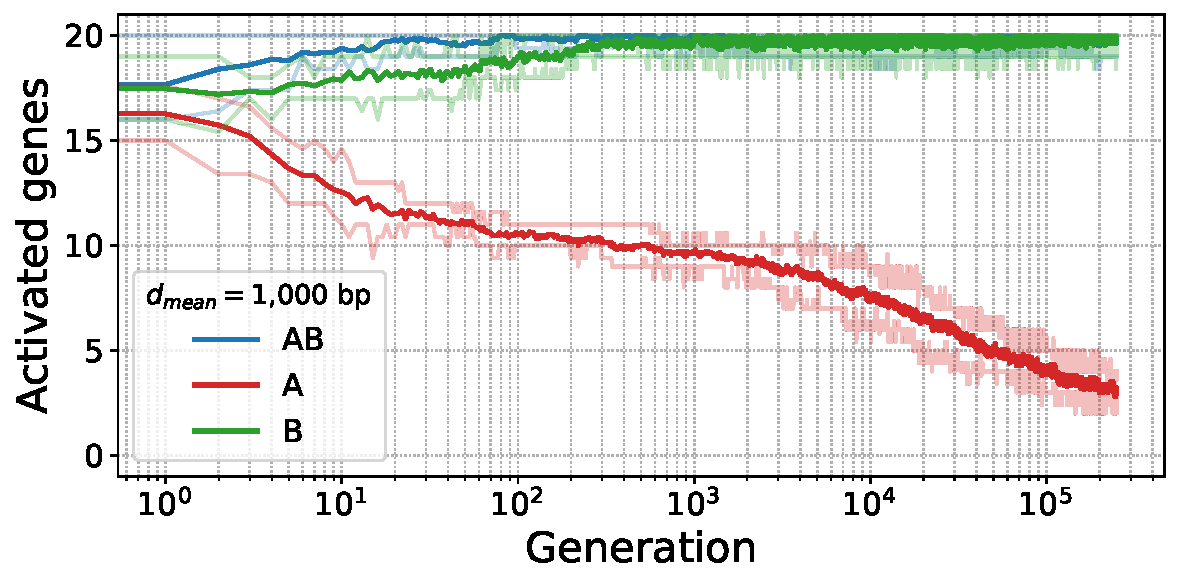
\includegraphics[width=0.495\textwidth]{param/mean-intergene/inter-1k/gene_activity_env_B.pdf}

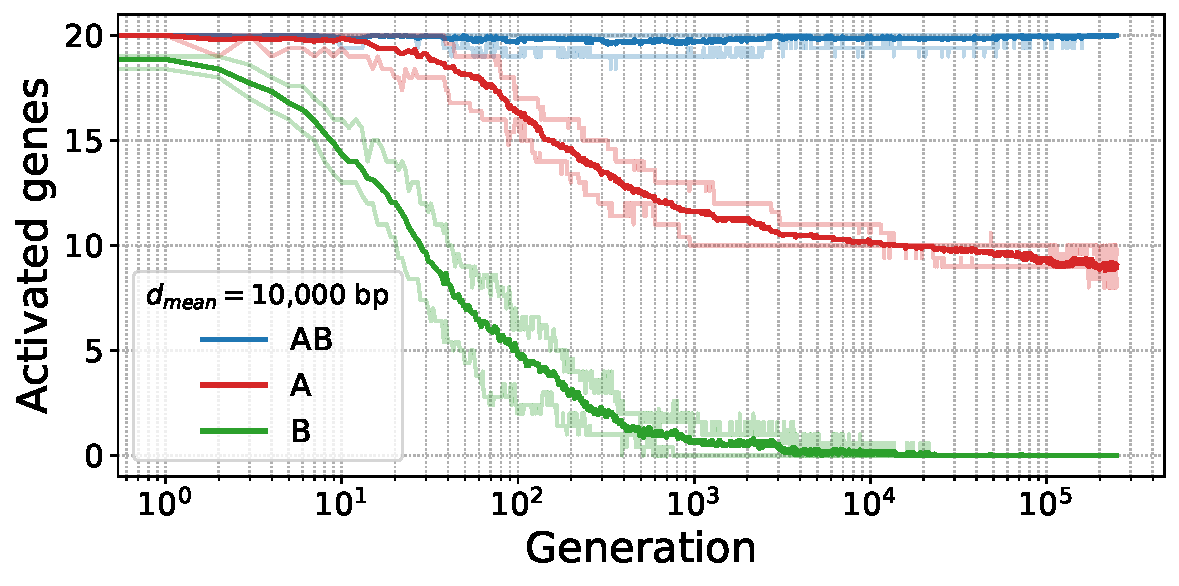
\includegraphics[width=0.495\textwidth]{param/mean-intergene/inter-10k/gene_activity_env_A.pdf}
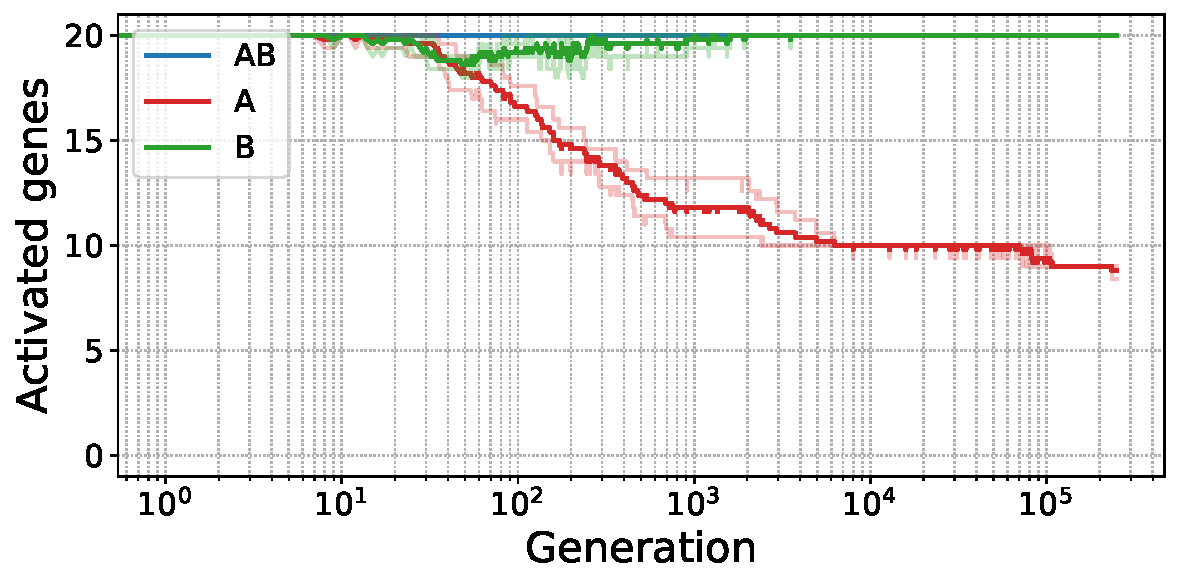
\includegraphics[width=0.495\textwidth]{param/mean-intergene/inter-10k/gene_activity_env_B.pdf}
\caption[Evolution of the number of activated genes in each environment, with increasing mean intergenic distances]{Average number of activated genes per gene type in environment A (left) and B (right) during evolution, for average intergenic sizes from top to bottom of 10 bp, 125 bp (main run), 1 kb, and 10 kb.
Lighter lines represent the first and last decile of the data.}
\label{fig:param:mean-intergene-activ-by-env}
\end{figure}

Figure~\ref{fig:param:mean-intergene-activ-by-env} shows the evolution of the number of activated genes for each gene type in each environment, with mean intergenic distances increasing from top to bottom, for 250,000 generations.
For intergenic distances of 10 bp and 1 kb, the number of activated genes converges towards the target in each environment, as in the main run (which has a mean intergenic distance of 125 bp).
For a mean intergenic distance of 10 kb, the behavior is however qualitatively different.
While \emph{AB} genes and \emph{B} genes evolve towards the correct activation state in each environment, the proportion of activated \emph{A} genes stays close to 50\% in each environment, showing that \emph{A} genes do not evolve a well-differentiated expression pattern depending on the environment.

\begin{figure}[H]
\centering
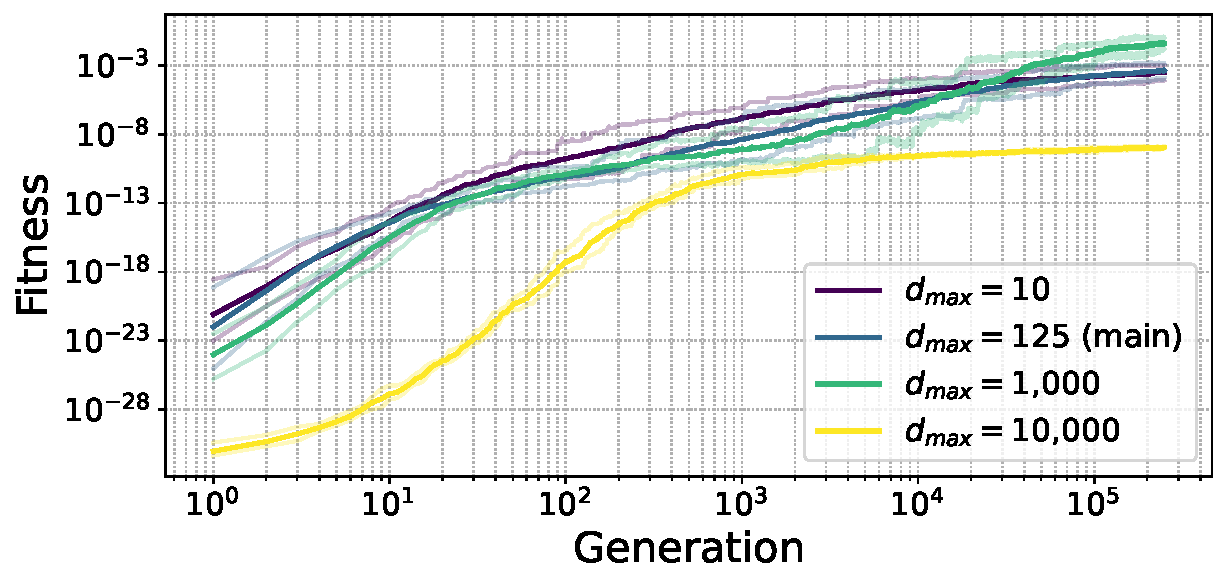
\includegraphics[width=0.8\textwidth]{param/mean-intergene/fitness_all_with_main.pdf}
\caption[Average fitness during evolution, with increasing mean intergenic distances]{Average fitness during evolution for average intergenic distances of 10 bp, 125 bp (main run), 1 kb, and 10 kb.
Lighter lines represent the first and last decile of the data.}
\label{fig:param:mean-intergene-fitness}
\end{figure}

Figure~\ref{fig:param:mean-intergene-fitness} shows the evolution of the average fitness of the best individual in each replicate of the simulations, for each value of the mean intergenic distance, including the main run for comparison.
It confirms the results seen in the previous figure: for intergenic distances from 10 bp to 1 kb, populations evolve successfully towards differentiated gene activation patterns.
For an intergenic size of 10 kb (in light blue), however, fitness increases much more slowly, and seems to converge towards a much smaller value.

\begin{figure}[H]
\centering
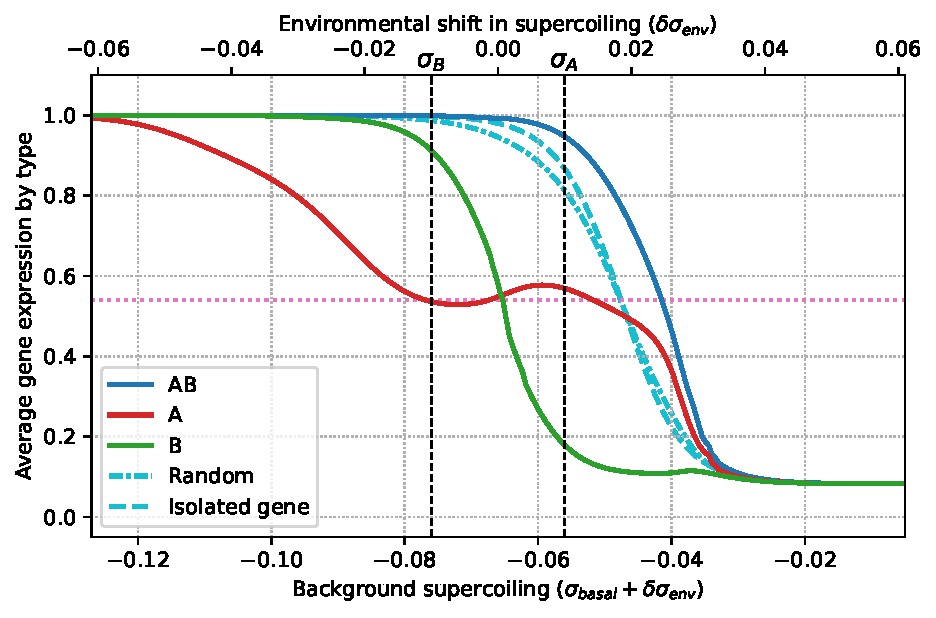
\includegraphics[width=0.9\textwidth]{param/mean-intergene/inter-10k/activity_sigmas_avg.pdf}
\caption[Average gene expression as a function of background supercoiling, with an intergenic distance of 10 kb]{Average gene expression as a function of background supercoiling, with an intergenic distance of 10 kb.}
\label{fig:param:mean-intergene-10kb-activ-by-sigma}
\end{figure}

Figure~\ref{fig:param:mean-intergene-10kb-activ-by-sigma} shows the average gene activity as a function of background supercoiling, for the best individual in each of the replicates with a mean intergenic distance of 10 kb.
In this case, we do not observe the clear relaxation-activated phenotype for \emph{A} genes that was present in the main simulation.
Instead, the average expression level of \emph{A} genes is indeed slightly lower in environment B than in environment A, but remains close to half expression for background supercoiling values between -0.08 and -0.05; on the contrary, both \emph{B} and \emph{AB} genes display expression curves that closely match their respective targets.
Note also that, with an intergenic distance of 10 kb, the average activity of genes on random genomes is almost identical to that of an isolated gene (as could be expected).

\begin{figure}[H]
\centering
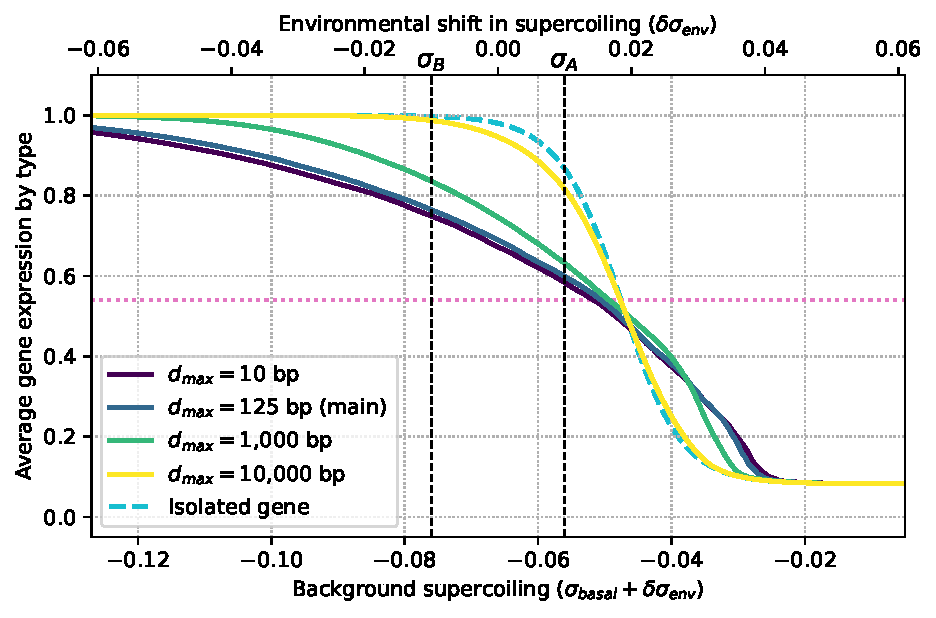
\includegraphics[width=0.9\textwidth]{param/mean-intergene/random_activ_per_sigma.pdf}
\caption[Average gene expression as a function of background supercoiling, with increasing mean intergenic distances, in random genomes]{Average gene expression as a function of background supercoiling in random genomes with increasing mean intergenic distances (full lines), and theoretical expression level of an isolated gene (dashed line).}
\label{fig:param:mean-intergene-random-activ-by-sigma}
\end{figure}

Figure~\ref{fig:param:mean-intergene-random-activ-by-sigma} shows the expression level as a function of background supercoiling for genes on random genomes with increasing mean intergenic distances.
For distances from 10 bp to 1 kb, the curves are qualitatively similar to one another, and quite different to the expression of an isolated, non-interacting genes.
In particular, gene expression levels are sensibly lower than the maximum in both environment A and environment B.
On the other hand, for a mean intergenic distance of 10 kb (in light blue), genes behave very closely to an isolated gene, and are all almost fully activated in both environments.
This behavior is also visible in Figure~\ref{fig:param:mean-intergene-activ-by-env} (bottom row) at the beginning of evolution, and explains the initially much lower fitness at an intergenic distance of 10 kb compared to the other values in Figure~\ref{fig:param:mean-intergene-fitness}.

Several hypotheses could explain the incomplete fulfillment of the evolutionary target in simulations with a mean intergenic distance of 10kb.
First, individuals begin evolution at a much lower fitness with a mean intergenic distance of 10 kb.
This initial impediment however does not explain why the number of activated \emph{A} genes remains similar in both environments throughout evolution, contrary to the other runs.
Another possible explanation could come from the mutational operator -- genomic inversions -- used during evolution.
As the endpoints of the genomic inversions are chosen by picking two bases uniformly at random in the intergenic regions, the number of fully neutral inversions increases with the size of these regions.
Indeed, if the two endpoint of an inversion fall in regions that are not within interaction distance of any gene, the inverted region does not interact with the rest of the genome, and the inversion is therefore completely neutral.
The increased proportion of neutral mutations when the intergenic distance is too large could make the exploration of the fitness landscape more difficult for populations, by creating hard to cross fitness valleys or plateaus between fitness peaks.
There is indeed no theoretical reason why genomes with large intergenic distances could not reach comparable fitnesses to the other intergenic distances in the mode, as a genome in which most of the intergenic content is compacted into a single intergenic region would have a qualitatively similar behavior, except for the few bordering genes on each side, to the same genome with a short intergenic region in the same position.

Evolution of gene regulation by supercoiling is therefore overall resilient to the range of gene densities seen in bacteria, but the evolution of relaxation-activated genes breaks down at the lower gene densities that are more characteristic of eukaryotes.


\section{Environmental Shift in Supercoiling}
\label{sec:param:sigma-env}

In the model, the environmental shifts in supercoiling $\sigma_A$ and $\sigma_B$ represent the effect of external stresses, such as salt shock, or pH or temperature changes, on the DNA supercoiling level, as they affect for example topoisomerase activity.
In this section, I tested the robustness of the evolution of differentiated expression levels when the shift in supercoiling caused by the environment $\sigma_A$ and $\sigma_B$ is 10 times and 100 times smaller than in the main run, i.e. when the stress is of a lower intensity.
The approach is similar to the one presented in Section~\ref{sec:alife:param_explor}, which however uses the proof-of-concept version of the model.

\begin{figure}[H]
\centering
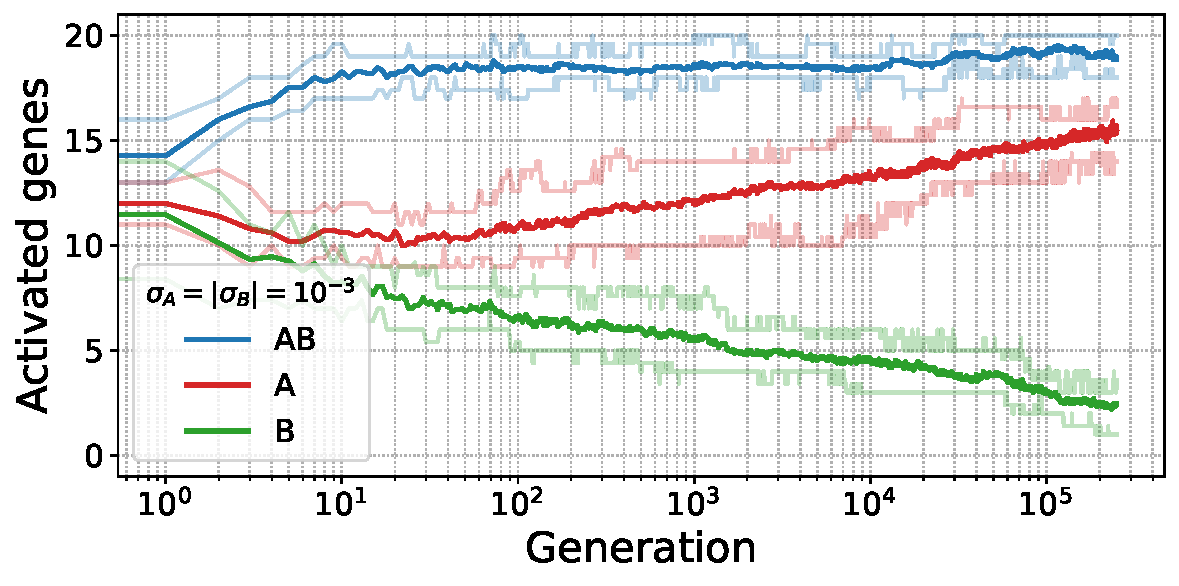
\includegraphics[width=0.495\textwidth]{param/sigma/sigma-1e-3/gene_activity_env_A.pdf}
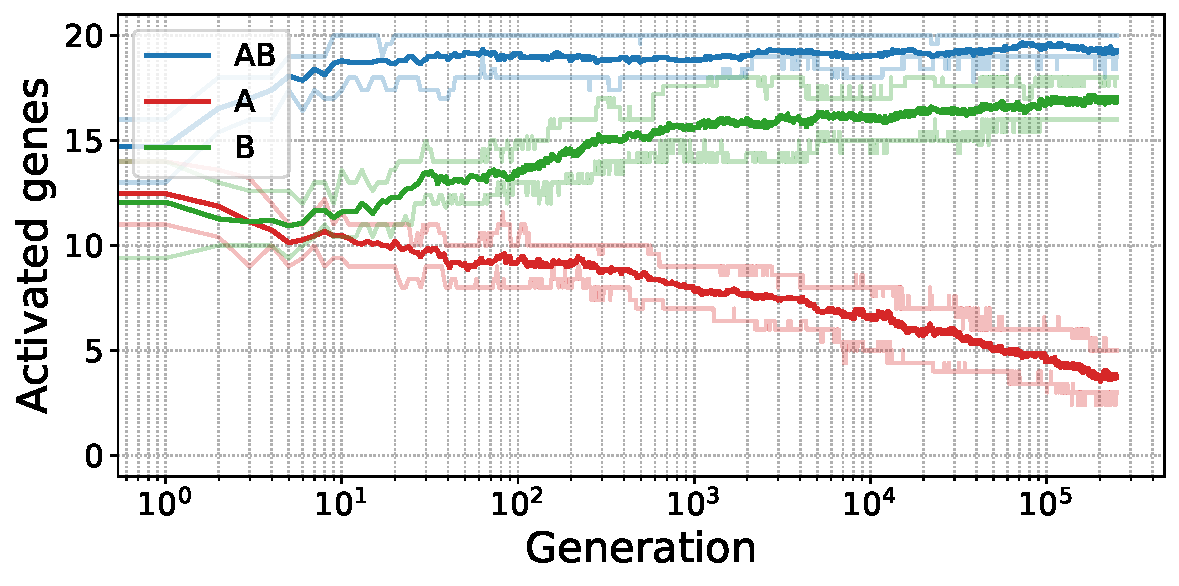
\includegraphics[width=0.495\textwidth]{param/sigma/sigma-1e-3/gene_activity_env_B.pdf}

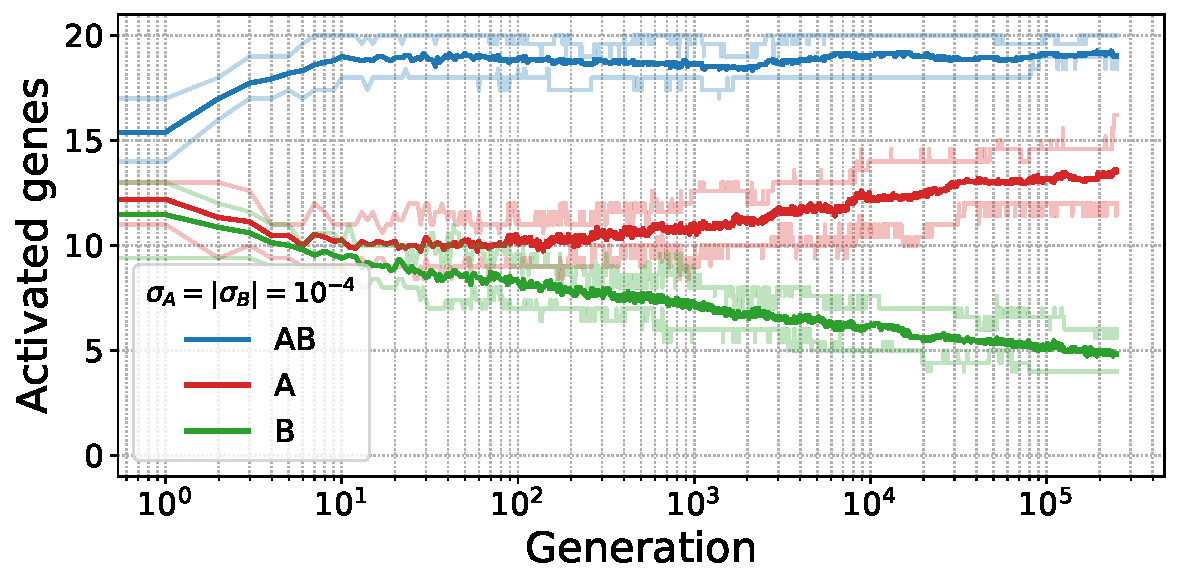
\includegraphics[width=0.495\textwidth]{param/sigma/sigma-1e-4/gene_activity_env_A.pdf}
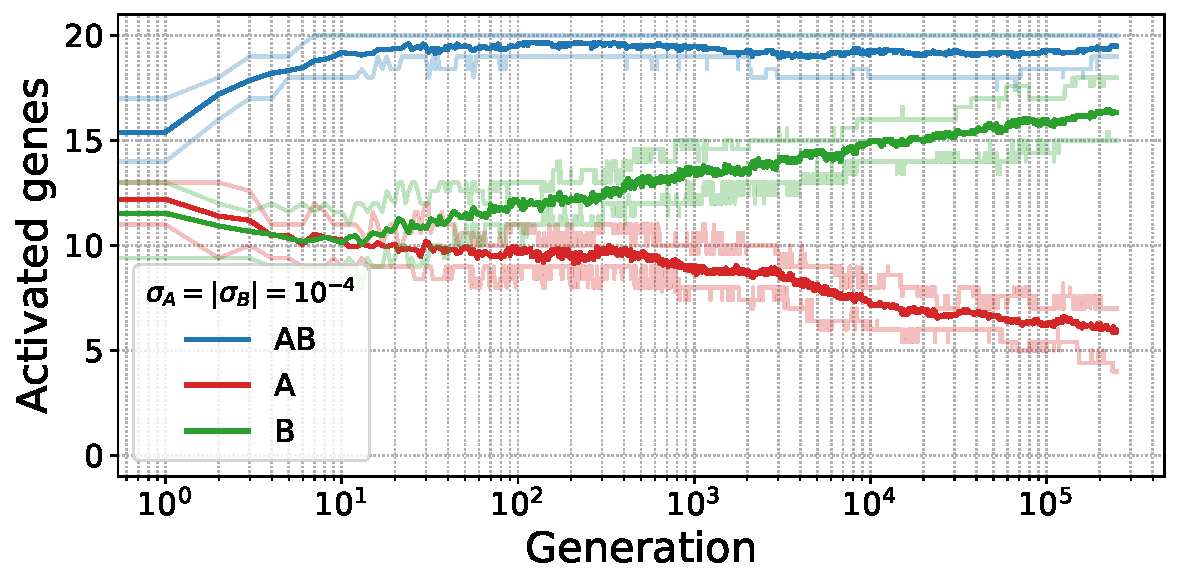
\includegraphics[width=0.495\textwidth]{param/sigma/sigma-1e-4/gene_activity_env_B.pdf}
\caption[Evolution of the number of activated genes in each environment, with decreasing environmental supercoiling shifts]{Evolution of the number of activated genes in environment A (left) and environment B (right), with environmental supercoiling shifts $\sigma_A = 10^{-3}$ and $\sigma_B = -10^{-3}$ (top) and $\sigma_A = 10^{-4}$ and $\sigma_B = -10^{-4}$ (bottom).
Lighter lines represent the first and last decile of the data.}
\label{fig:param:sigma-activ-by-env}
\end{figure}

Figure~\ref{fig:param:sigma-activ-by-env} shows the evolution of the number of activated genes for each gene type in each environment, with environmental shifts in supercoiling 10 times smaller than the main run (top) and 100 times smaller (bottom), for 250,000 generations.
In both cases, differentiated gene expression patterns evolve, although evolution seems to be slower when $\sigma_A$ and $\sigma_B$ are 100 times smaller than in the main run.
This shows that evolution of different gene expression levels as a response to externally-induced perturbations in the supercoiling level can therefore take place even when these perturbations are very minute compared to translation-generated supercoiling, and reinforces the plausibility of the hypothesis that DNA supercoiling can be used as an sensory device for the regulation of gene expression in response to environmental stress.

\begin{figure}[H]
\centering
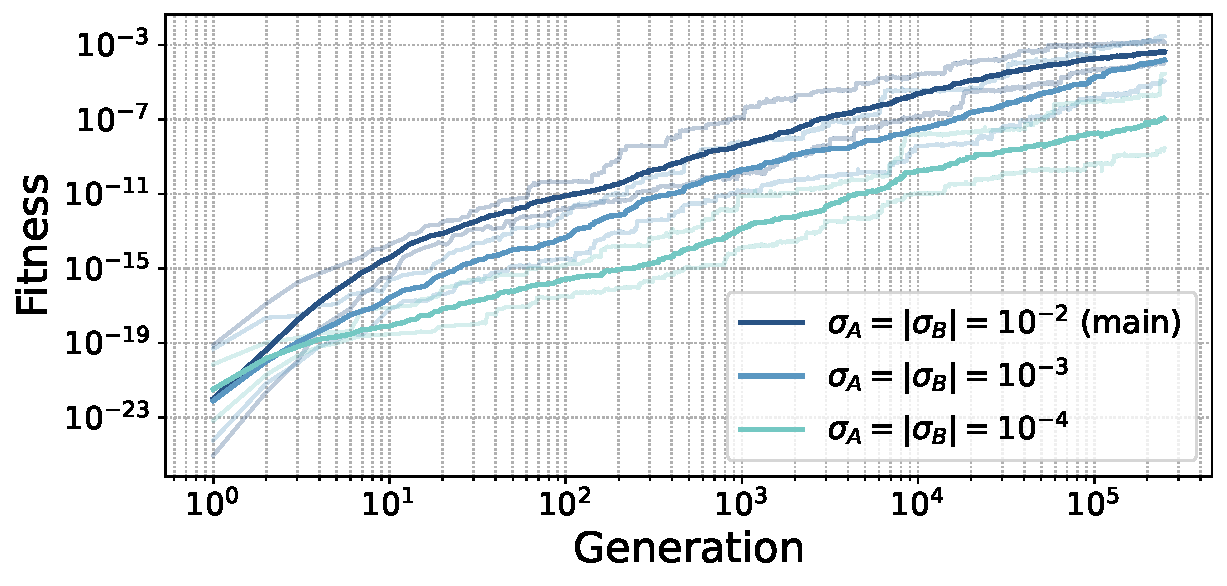
\includegraphics[width=0.8\textwidth]{param/sigma/fitness_all_with_main.pdf}
\caption[Average fitness during evolution, with decreasing environmental supercoiling shifts]{Average fitness during evolution, with environmental shifts in supercoiling logarithmically decreasing in absolute value: $\sigma_A = 10^{-2}$ and $\sigma_B = -10^{-2}$ (main run), $\sigma_A = 10^{-3}$ and $\sigma_B = -10^{-3}$ (10 times smaller than in the main run) and $\sigma_A = 10^{-4}$ and $\sigma_B = -10^{-4}$ (100 times smaller than the main run).
Lighter lines represent the first and last decile of the data.}
\label{fig:param:sigma-fitness}
\end{figure}

Figure~\ref{fig:param:sigma-fitness} shows the evolution of the average fitness of the best individual in each replicate, for each pair of environmental supercoiling values.
It confirms the results seen in the previous figure: fitness keeps increasing throughout the simulation in all cases, but more slowly when the environmental perturbation is the smallest.

\begin{figure}[H]
\centering
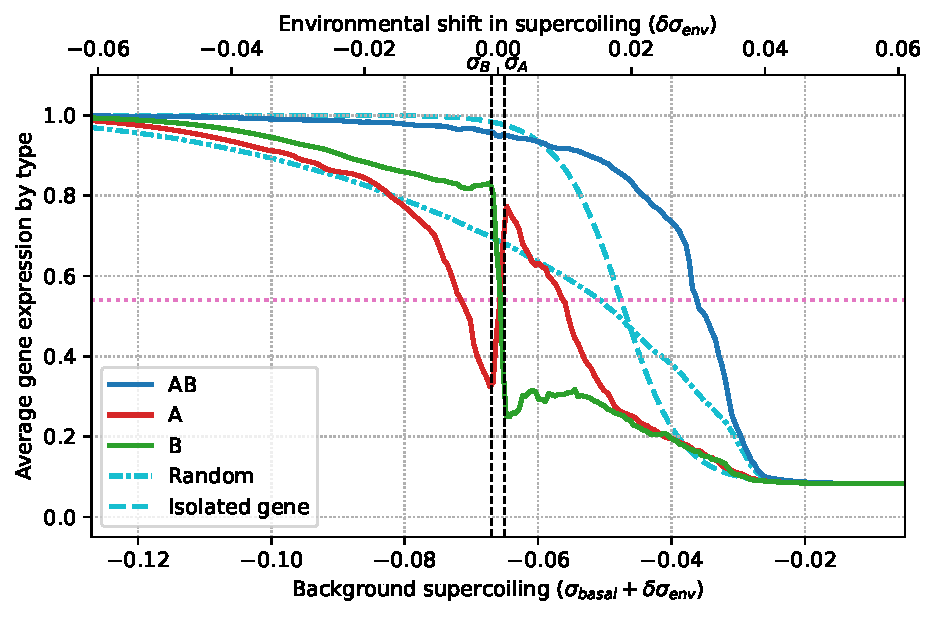
\includegraphics[width=0.9\textwidth]{param/sigma/sigma-1e-3/activity_sigmas_avg.pdf}
\caption[Average gene expression as a function of background supercoiling, with an absolute environmental supercoiling shift of 0.001]{Average gene expression as a function of background supercoiling, with environmental supercoiling shifts $\sigma_A = 10^{-3}$ and $\sigma_B = -10^{-3}$.}
\label{fig:param:sigma-1e-3-activ-by-sigma}
\end{figure}

Figure~\ref{fig:param:sigma-1e-3-activ-by-sigma} shows the average gene expression per gene type as a function of background supercoiling, for the best individuals at the end of evolution with environmental shifts in supercoiling of $\sigma_A = 10^{-3}$ and $\sigma_B = -10^{-3}$.
Even though the difference between the two environments is 10 times smaller than in the main run, \emph{A} genes are still able to evolve a relaxation-activated phenotype, and \emph{B} genes are still able to quickly transition from high activation to high inhibition in a much shorter range of supercoiling values.

\begin{figure}[H]
\centering
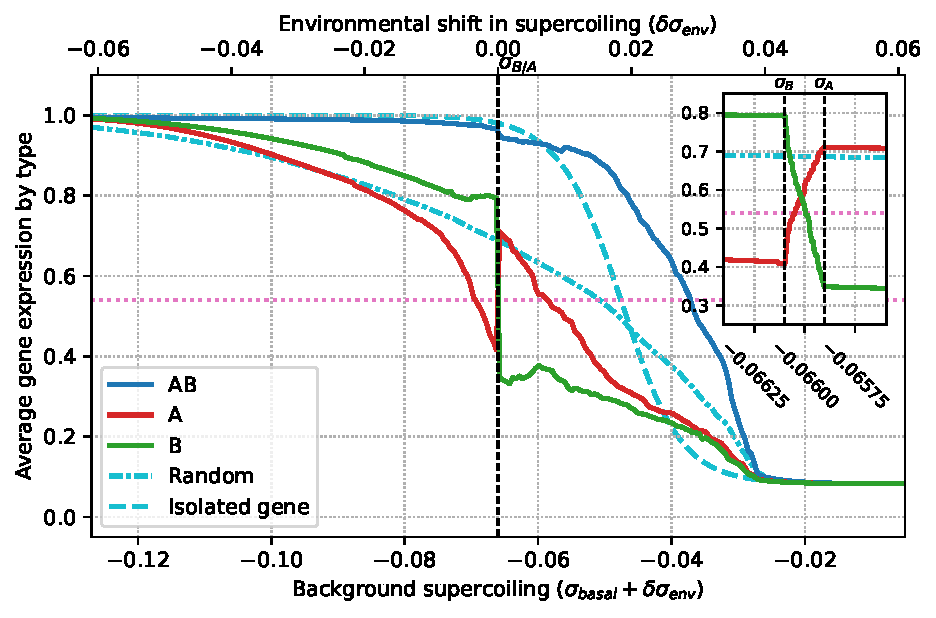
\includegraphics[width=0.9\textwidth]{param/sigma/sigma-1e-4/activity_sigmas_avg.pdf}
\caption[Average gene expression as a function of background supercoiling, with an absolute environmental supercoiling shift of 0.0001]{Average gene expression as a function of background supercoiling, with environmental supercoiling shifts $\sigma_A = 10^{-4}$ and $\sigma_B = -10^{-4}$.
The inset at the top right of the figure shows a 150x zoom on supercoiling shift values near zero.}
\label{fig:param:sigma-1e-4-activ-by-sigma}
\end{figure}

Figure~\ref{fig:param:sigma-1e-4-activ-by-sigma} similarly shows average gene expression per gene type as a function of background supercoiling, this time with environmental supercoiling shifts $\sigma_A = 10^{-4}$ and $\sigma_B = -10^{-4}$.
Strikingly, \emph{A} genes and \emph{B} genes are still able to evolve different expression levels in the two environments, even though they are 100 times closer than in the original experiment (see the inset for the precise expression levels between $\sigma_B$ and $\sigma_A$).
Even when the environments have an effect that is around 100 times smaller than the transcription-generated supercoiling (see Figure~\ref{fig:ploscb:genomes} for an example genome and the associated transcription-generated supercoiling values), the gene regulatory networks that evolve in the simulations are still able to separate the different environments and lead gene expression levels to very different states.

These results further confirm the results of the parametric exploration of the proof-of-concept version of \emph{EvoTSC}, at the end of Chapter~\ref{chap:alife}.
They show that perturbations that have little to no effect either on an isolated gene, or on a random genome (averaging over every gene), can be picked up and amplified by supercoiling-mediated gene regulatory networks, and result in clearly differentiated gene expression levels.


\section{Number of Genes}
\label{sec:param:300-genes}

All the simulations presented up to now were run with $n = 60$ genes on the genomes of individuals.
Although genes in our model correspond to transcriptional units, and could describe operons that contain multiple genes, this number remains much lower than the real number of genes in bacteria, which ranges from the 482 protein-coding genes found in \emph{Mycoplasma genitalium}, the bacteria with the smallest-known genome~\citep{glass2006}, up to over 9,000 predicted genes in \emph{Sorangium cellulosum}~\citep{schneiker2007}.
At first sight, increasing the total number of genes in the model should not qualitatively change the simulation results, as with a genome size of 60, genes already only interact via the transcription-supercoiling coupling with a small proportion of the genome.
In order to verify this hypothesis, I ran simulations with $n = 300$ genes, with maximum supercoiling interaction distances of $d_{max} =$ 5~kb (the value used in the main runs) and $d_{max} =$ 25 kb.
As the algorithmic complexity of the \emph{EvoTSC} scales quadratically with the number of genes, the simulations were run for 100,000 generations only to keep their execution time manageable, but the simulations already show qualitative results by that time.

\begin{figure}[H]
\centering
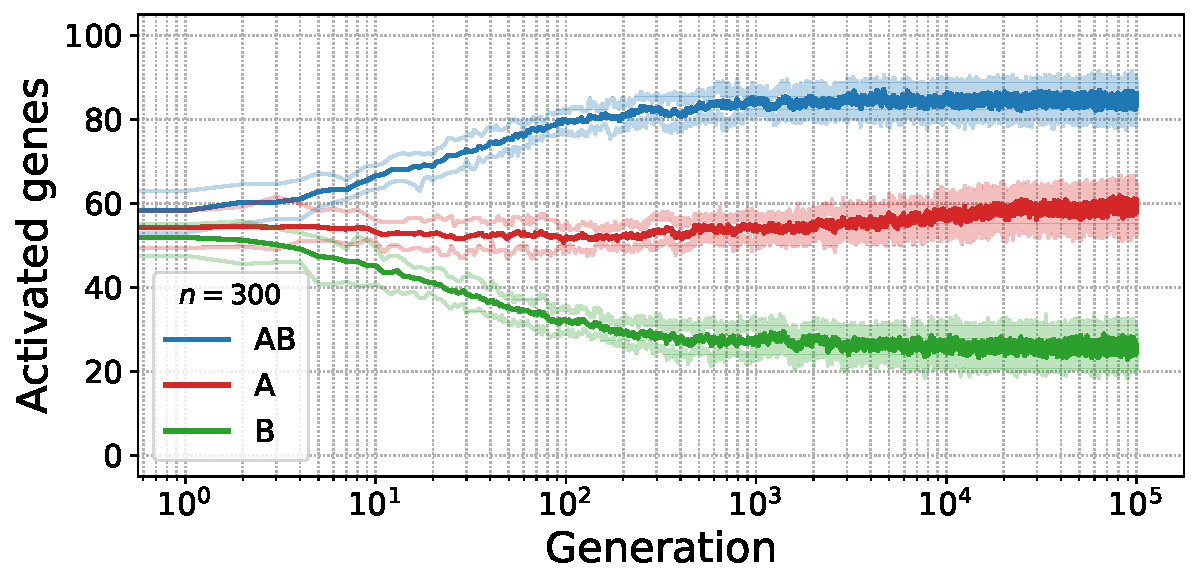
\includegraphics[width=0.495\textwidth]{param/300-genes/interaction-5k/gene_activity_env_A.pdf}
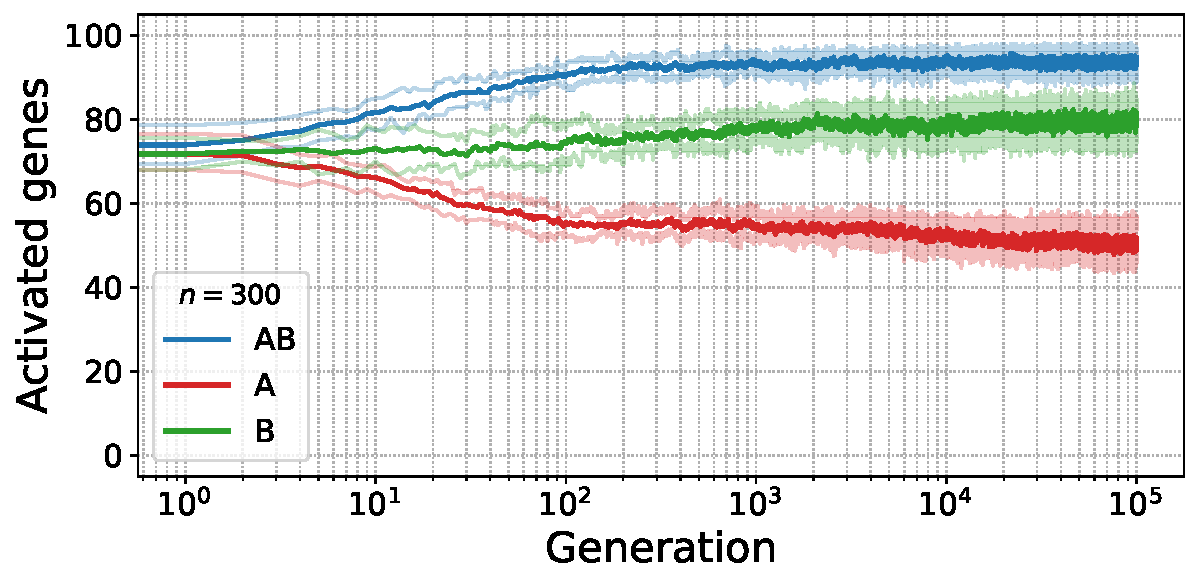
\includegraphics[width=0.495\textwidth]{param/300-genes/interaction-5k/gene_activity_env_B.pdf}

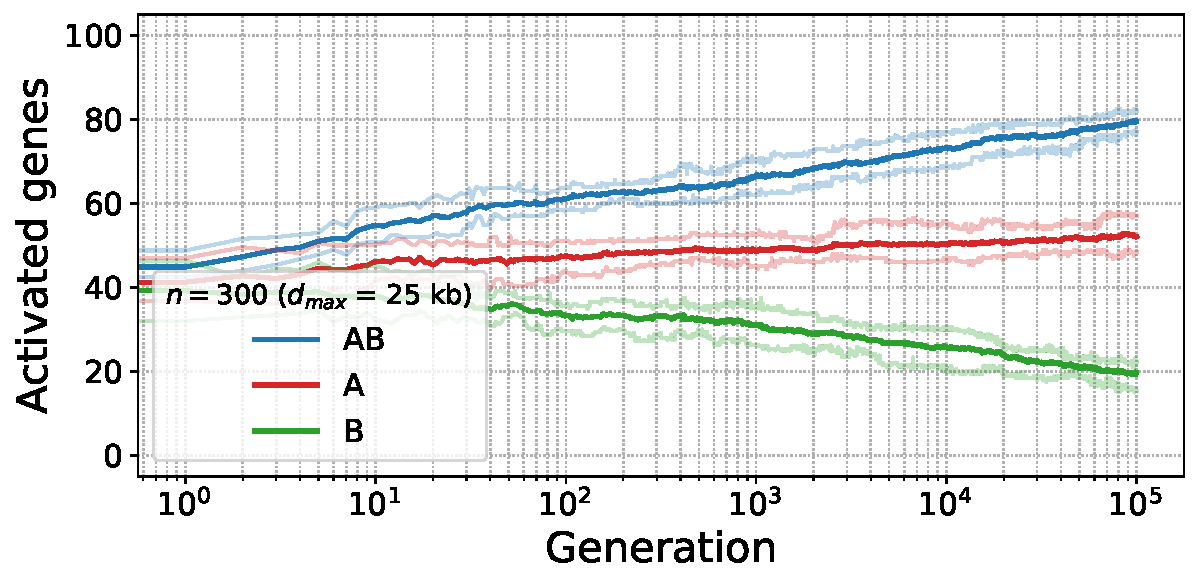
\includegraphics[width=0.495\textwidth]{param/300-genes/interaction-25k/gene_activity_env_A.pdf}
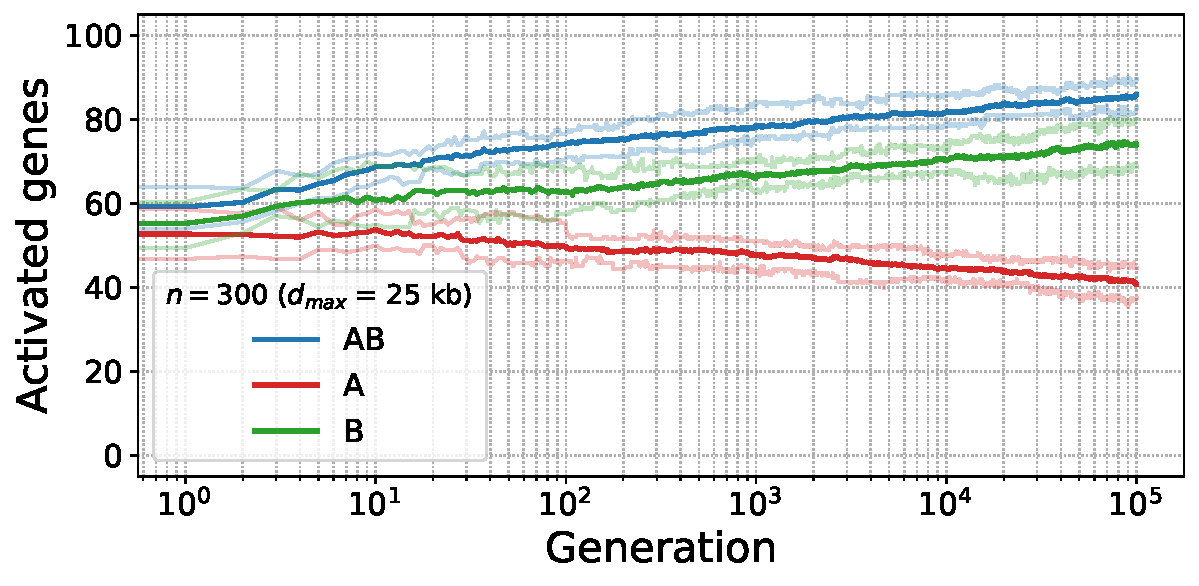
\includegraphics[width=0.495\textwidth]{param/300-genes/interaction-25k/gene_activity_env_B.pdf}
\caption[Evolution of the number of activated genes in each environment, with a 300-gene genome]{Evolution of the number of activated genes in environment A (left) and environment B (right), with a genome containing 300 genes, and an interaction distance of 5 kb (top) and 25 kb (bottom).
Lighter lines represent the first and last decile of the data.}
\label{fig:param:300genes-activ-by-env}
\end{figure}

Figure~\ref{fig:param:300genes-activ-by-env} shows the evolution of the number of activated genes of each type in each environment, for populations of individuals with a 300-gene genome, for 100,000 generations.
While these simulations lasted only for 100,000 simulations, the evolutionary trajectories are already different from the ones taken by the main run (in Figure~\ref{fig:ploscb:gene_activity_by_env}).
Different numbers of activated genes evolve in each case as a function of the environment supercoiling, but the patterns differ depending on the interaction distance.
With the shorter interaction distance, the number of activated genes of each type seems to plateau after about 10,000 generations (top).
On the contrary, evolution seems to continue by the end of the runs for the wider interaction distance (bottom).

\begin{figure}[H]
\centering
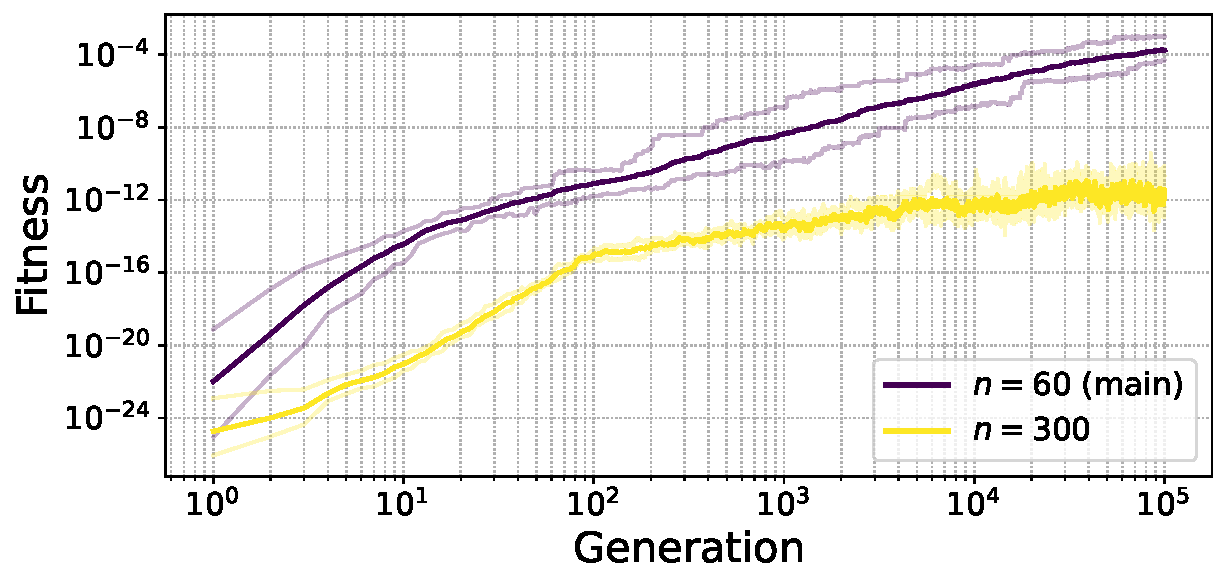
\includegraphics[width=0.8\textwidth]{param/300-genes/fitness_all_with_main.pdf}
\caption[Average fitness during evolution, with a 300-gene genome]{Average fitness during evolution, with a 300-gene genome, and an interaction distance of 5 kb or 25 kb.
Lighter lines represent the first and last decile of the data.}
\label{fig:param:300gene-fitness}
\end{figure}

Figure~\ref{fig:param:300gene-fitness} shows the evolution of the average fitness of the best individual in each replicate of the simulations with 300 genes per individual, compared to the main run.
As expected given the high proportion of \emph{A} genes with an incorrect activation state in each environment that is visible in both sets of simulations in Figure~\ref{fig:param:300genes-activ-by-env}, the fitness of the runs with 300 genes remains much lower than the fitness of the main runs throughout evolution.
Moreover, the fitness trajectory in the runs with 300 genes also depends on the interaction distance, in accordance with the evolution of the number of activated genes in each environment presented above.
For an interaction distance of 5 kb, fitness indeed seems to plateau at a much lower value than the main run by the end of the 100,000 generations, while it keeps on steadily increasing for an interaction distance of 25 kb.

Figure~\ref{fig:param:300genes-activ-by-sigma} shows the average expression of genes for each gene type as a function of the background supercoiling level, for interaction distances of 5 kb (top) and 25 kb (bottom).
In both cases, and similarly to the simulation with a 10 kb intergenic distance, \emph{A} genes do not seem to meaningfully evolve a relaxation-activated phenotype by the end of the simulations.
With 300 genes, the response of each gene type seems to diverge less from the behavior of genes on a random genome than in the other simulations presented above.
In particular, with an interaction distance of 5 kb, the average activity of \emph{A} genes is above the activation threshold at $\sigma_B$ (i.e., in environment B), in contrast to all the other experimental settings except when the mean intergenic distance is 10 kb (Figure~\ref{fig:param:mean-intergene-10kb-activ-by-sigma}).
With an interaction distance of 25 kb, the average expression of \emph{A} genes on the contrary goes below the activation threshold at $\sigma_B$ and above the threshold at $\sigma_A$, which correlates with the higher fitness observed for this value of the intergenic distance.

\begin{figure}[H]
\centering
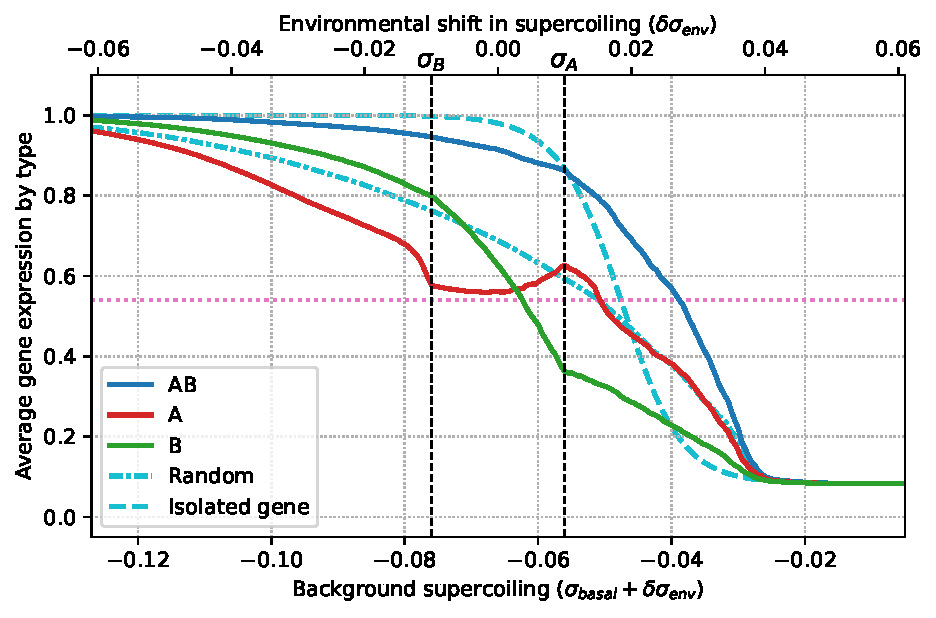
\includegraphics[width=0.9\textwidth]{param/300-genes/interaction-5k/activity_sigmas_avg.pdf}
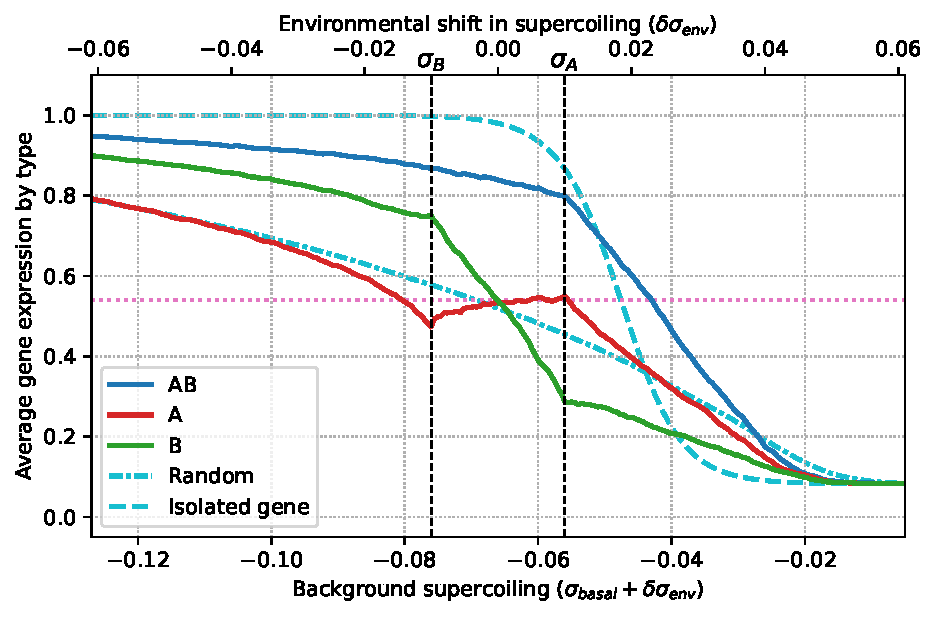
\includegraphics[width=0.9\textwidth]{param/300-genes/interaction-25k/activity_sigmas_avg.pdf}
\caption[Average gene expression as a function of background supercoiling, with a 300-gene genome]{Average gene expression as a function of background supercoiling, with a 300-gene genome and an interaction distance of 5 kb (top) and 25 kb (bottom).}
\label{fig:param:300genes-activ-by-sigma}
\end{figure}

A possible hypothesis for the slower evolution of the runs with $n =$ 300 genes lies in the much larger size of the fitness landscape to explore during evolution through genomic inversions, and in the combinatorics of these inversions.
As an inversion is defined by two points chosen on the genome, the number of different inversions grows with the square of its size; if we disregard the role of the intergenic sequences (which have an average length of 125 bp in all the runs in this section), this number grows with the square of the number of genes.
The number of inversions to explore in order to find beneficial relative gene positions could therefore be much higher in larger genomes; as the number of inversions does not depend on genome size, larger genomes could take more time to explore the fitness landscape.
A second hypothesis also depends on the number of genes affected by inversions, but in a slightly different way.
As the end points of genomic inversions are chosen at random, the average size of an inversion is of half the genome with all parameter values, but the absolute distance between the end points of the inversion changes with the number of genes on the genome.
In larger genomes, the genes located near one of the end points of an inversion are therefore further apart from the genes located near the other end point of the inversion, and could therefore be more rarely part of the same gene regulatory network than in smaller genomes.
In particular, inversions affecting only a few genes could be rarer, making it more difficult to locally adjust gene regulatory networks, even though the relative orientation of neighbors and local networks play an important role (see Chapter~\ref{chap:ploscb}).
This would in particular explain why the runs with 300 genes but a larger interaction distance evolve better, as the breadth of the regulatory networks increases with the interaction distance.

A further investigation of the behavior of the model with larger number of genes could therefore seem warranted, but the overall qualitative evolution of different gene activation levels in response to environmental perturbations remains present when increasing the number of genes on the genome in the model, at least when the interaction distance is large.


\section{Introducing Indels}
\label{sec:param:evolve-intergene}

In Section~\ref{sec:param:mean-intergene}, we saw that the evolution of differentiated gene expression patterns depends on the mean intergenic distance: at low to intermediate values (akin to bacterial genomes), genes present environment-specific activity levels, while \emph{A} genes fail to do so at the largest tested intergenic distance (akin to eukaryotic genomes).
In order to understand more finely the role of intergenic distances in the evolution of the regulatory networks underpinning these expression patterns, I introduced a new mutational operator which allows these distances to evolve, through the addition or deletion of a small number of bases between genes (indels).
The last set of simulations presented in this chapter tackle the exploration of the model with this additional mutational operator.

In order to perform an indel in the model, we first pick a number of base pairs to add or delete, by drawing from a normal distribution $\mathcal{N}(0, s^2)$, with $s^2 = $ 10.
Then, we draw uniformly at random a gene, and add or remove the corresponding number of bases from the intergenic section starting immediately after that gene, in the forward direction.
If the intergenic section is too small to delete the chosen number of base pairs, we try drawing another gene at random, before giving up after a certain number of tries.
For these simulations, I ran 15 replicates for 1,000,000 generations (as in the main runs in Chapter~\ref{chap:ploscb}), in order to allow for the mean intergenic distance to converge.
The initial value of the mean intergenic distance was set to 125 bp, in order to match the main set of simulation.

\begin{figure}[H]
\centering
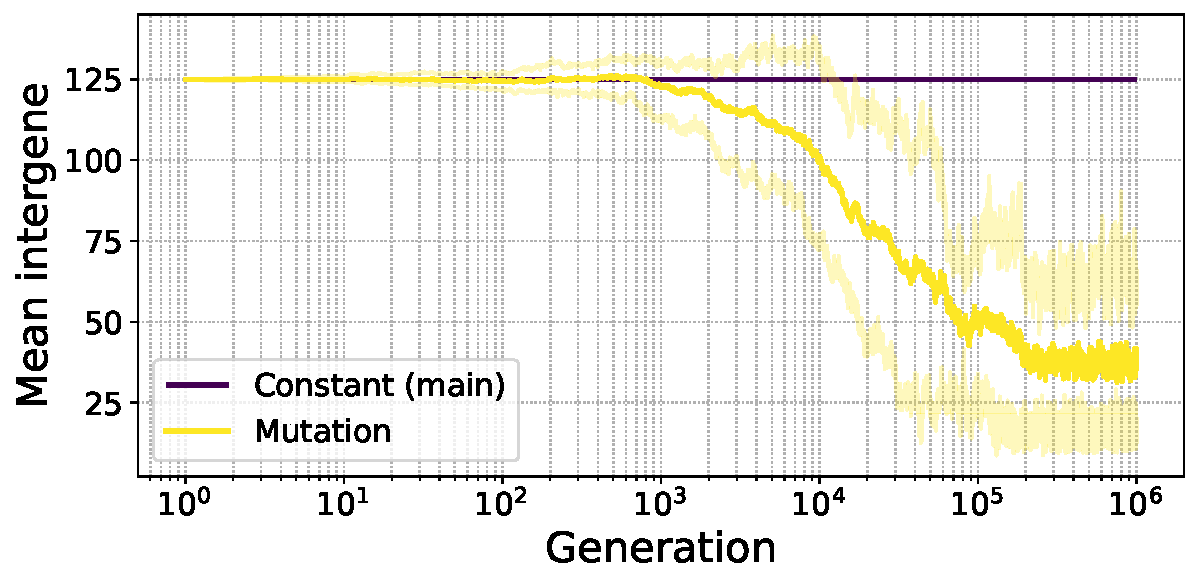
\includegraphics[width=0.8\textwidth]{param/evolve-intergene/intergenic_size_all.pdf}
\caption[Average intergenic size during evolution, with indels]{Average intergenic distance during evolution with indels, compared with the constant average intergenic distance in the main run.
Lighter lines represent the first and last decile of the data.}
\label{fig:param:evolve-intergene-intergene}
\end{figure}

Figure~\ref{fig:param:evolve-intergene-intergene} show the evolution of the mean intergenic distance, averaged over the best individual of each replicate, at every generation, compared to the initial value of 125 bp.
The average intergenic distance actually decreases during evolution, and seems to converge to a value of around 40 bp.
This result is opposite to what could have been expected, as the highest fitness when varying intergenic distances is actually reached for a value of 1 kb (Figure~\ref{fig:param:mean-intergene-fitness}).
There therefore seems to be a selection pressure towards reducing intergenic distances through indels, even though this does not lead to the highest attainable fitness.

\begin{figure}[H]
\centering
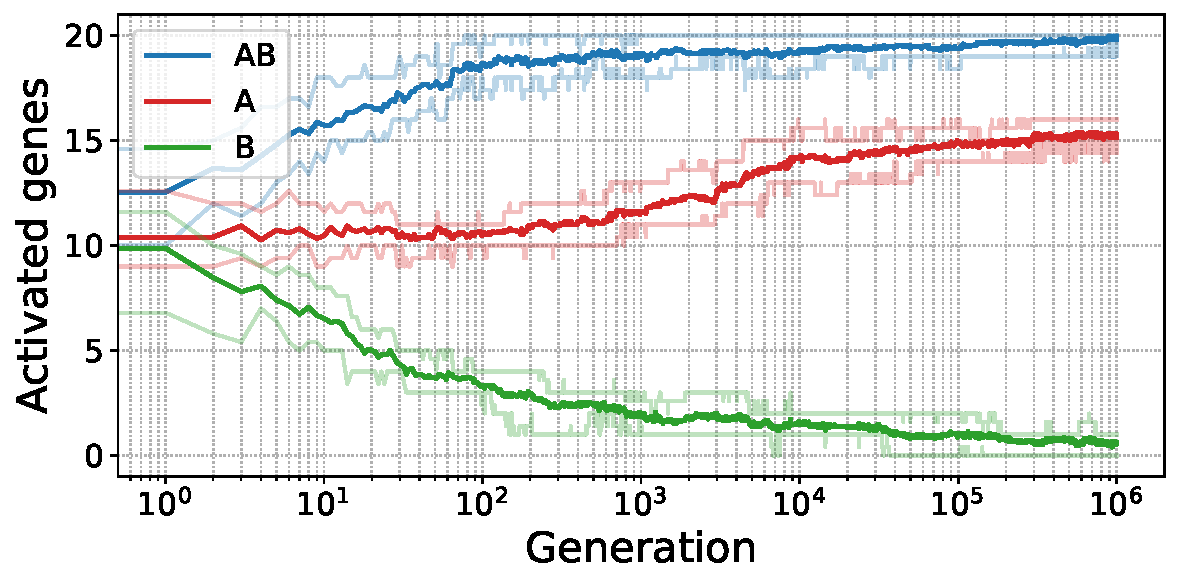
\includegraphics[width=0.495\textwidth]{param/evolve-intergene/gene_activity_env_A.pdf}
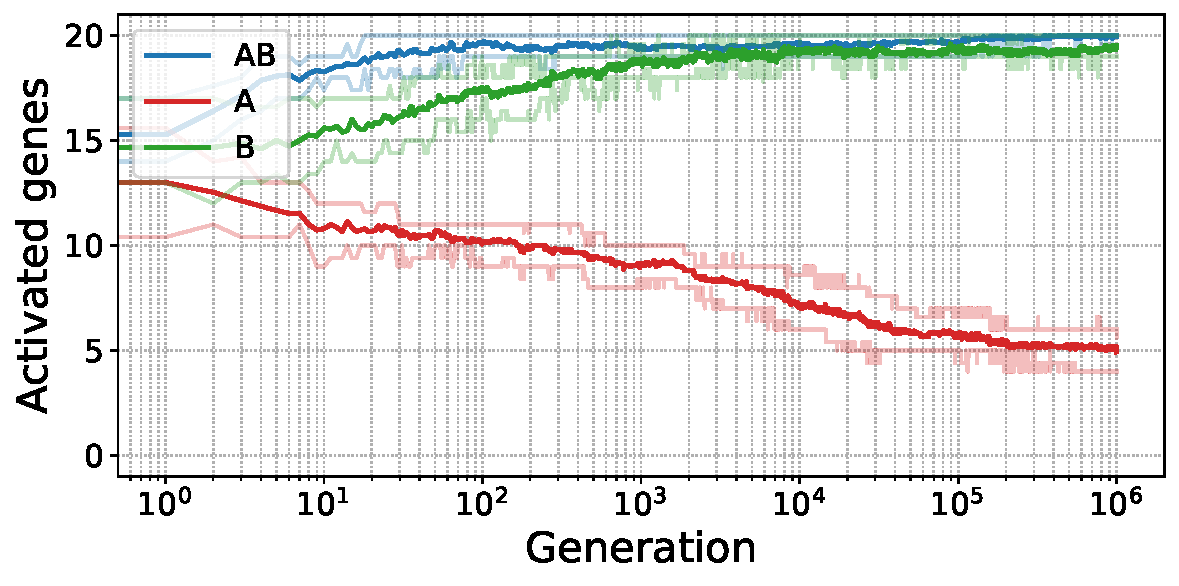
\includegraphics[width=0.495\textwidth]{param/evolve-intergene/gene_activity_env_B.pdf}
\caption[Evolution of the number of activated genes in each environment, with indels]{Evolution of the number of activated genes per gene type in environment A (top) and environment B (bottom), with indels.
Lighter lines represent the first and last decile of the data.}
\label{fig:param:evolve-intergene-activ-by-env}
\end{figure}

Figure~\ref{fig:param:evolve-intergene-activ-by-env} shows the evolution of the number of activated genes of each type, in each environment.
Similarly to the main run, differentiated expression levels evolve in the two environments, with in particular around 75\% of \emph{A} genes activated in environment A and 75\% of \emph{A} genes inhibited in environment B.

\begin{figure}[H]
\centering
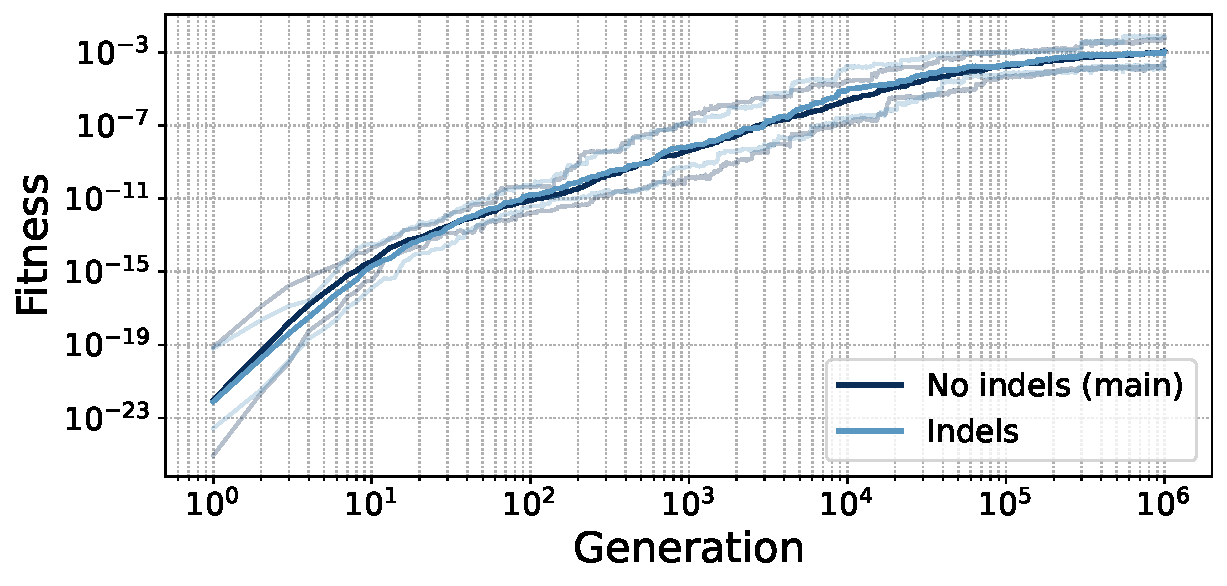
\includegraphics[width=0.8\textwidth]{param/evolve-intergene/fitness_all_with_main.pdf}
\caption[Average fitness during evolution, with indels]{Average fitness during evolution, with indels and without indels (main run).
Lighter lines represent the first and last decile of the data.}
\label{fig:param:evolve-intergene-fitness}
\end{figure}

Figure~\ref{fig:param:evolve-intergene-fitness} shows the average fitness during evolution of the individuals in the simulations with intergenic distance mutations, compared to the main simulations.
As in the runs with an intergenic distance of 10 bp (in Figure~\ref{fig:param:mean-intergene-fitness}), evolution progresses quite similarly to the main run.
Consistently with the observed evolution of the mean intergenic distance, but still surprisingly as evolution towards higher intergenic distances could be possible, populations with indels attain a lower fitness after 1,000,000 generations ($1.12\cdot10^{-3}$) than populations with a constant mean intergenic distance of 1 kb after 250,000 generations ($3.78\cdot 10^{-2}$).

\begin{figure}[H]
\centering
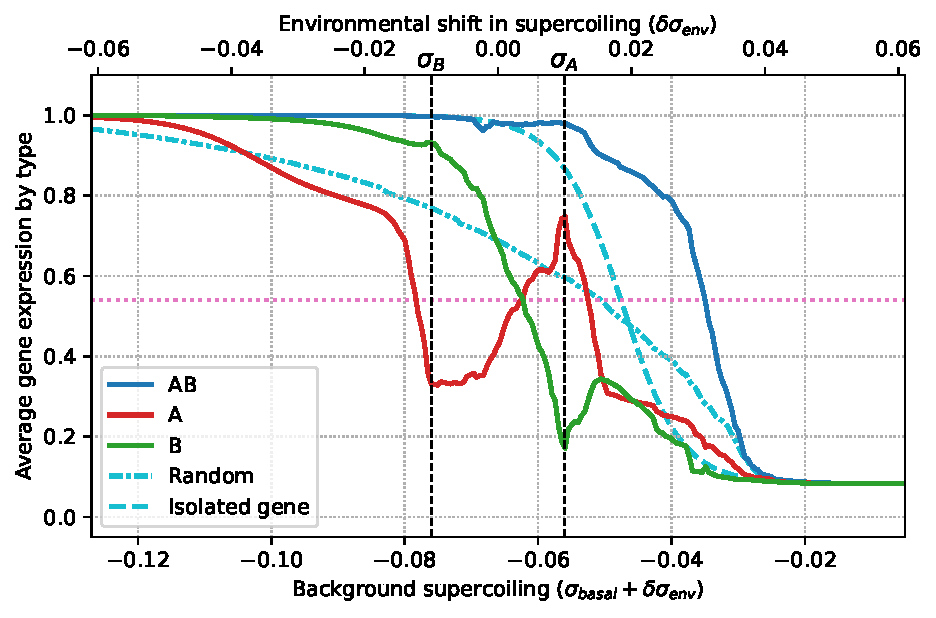
\includegraphics[width=0.9\textwidth]{param/evolve-intergene/activity_sigmas_avg.pdf}
\caption[Average gene expression as a function of background supercoiling, with indels]{Average gene expression for each gene type type as a function of background supercoiling, with indels.}
\label{fig:param:evolve-intergene-activ-by-sigma}
\end{figure}

Finally, Figure~\ref{fig:param:evolve-intergene-activ-by-sigma} shows the average gene activity for each gene type as a function of background supercoiling, for the simulations with indels.
Consistently with the results obtained in Section~\ref{sec:param:mean-intergene}, we can see that \emph{A} genes display a relaxation-activated phenotype.

These results seem to suggest that, even though evolving towards higher intergenic distances would allow populations to reach greater fitnesses, there is a stronger selection pressure that keeps intergenic distances at a low value.
As in section~\ref{sec:param:300-genes}, this selection pressure could be related to the combinatorics of genomic inversions.
As the number of different inversions grows quadratically with the number of intergenic bases, reducing the mean intergenic distance diminishes the size of the evolutionary space that is available through genomic inversions.
If beneficial inversions happen more often in individuals with reduced genomes than with larger genomes, that is if the evolvability of reduced genomes is higher than that of larger genomes, then a small mean intergenic distance could provide a short-term evolutionary advantage even though it leads to a lower fitness peak in the long term.
Although this hypothesis warrants further investigation, these results could be interpreted as an indirect conflict between direct selection favoring a higher-dimensional fitness landscape with higher peaks, and indirect selection favoring a lower-dimensional fitness landscape with more easily reachable peaks.


\section{Discussion}

The simulations carried out with the different parameter values presented above show that the results obtained with the model are overall quite robust, as differentiated gene expression by type and environment evolve over a wide range of biologically relevant values.
In particular, these results are robust with regard to the size of topological domains, which corresponds to the maximum interaction distance for the transcription-supercoiling coupling and has been given different experimental values; to the mean intergenic distance, in a range that is representative of the bacterial species; and to the intensity of changes in the background supercoiling that represent environmental sources of stress.
The gene regulatory networks that evolve in the model can indeed differentiate between environments that create much smaller levels of supercoiling than generated by transcription itself.

Overall, changing the value of each parameter in the model has two main consequences.
The first -- direct -- consequence is to affect the phenotype of individuals, by modulating the effect of the transcription-supercoiling coupling on gene expression (for example, by increasing the number of neighbors a gene interacts with).
This direct effect is illustrated in Figures~\ref{fig:param:inter25k-random-activ-by-sigma} and~\ref{fig:param:mean-intergene-random-activ-by-sigma}.
The second -- indirect -- consequence is to change the structure of the fitness landscape that underlies the possible evolutionary trajectories, by possibly affecting its dimension, its ruggedness, or the number and proportion of beneficial, neutral, or deleterious mutations.
This indirect effect is illustrated in Figures~\ref{fig:param:mean-intergene-fitness} and~\ref{fig:param:300gene-fitness}.
The fact that genomes with a higher number of genes or intergenic distances (above 10 kb) are not able to evolve a fitness as high as that of the smaller genomes exemplifies the strength of this second effect.
Indeed, as the number of available mutations using the mutational operator of genomic inversions scales quadratically with the number of base pairs on the genome (as described above), the proportion of possible genotypes that can be explored over a given number of generations with a constant number of individuals diminishes with as genome size increases.
In order to quantify this effect, an interesting experiment would be to run additional simulations in which every length-related parameter (maximum interaction distance, mean intergenic distance, and gene length) is scaled down by the same factor.
This would allow us to control the number of available mutations and therefore the speed of evolution, but should in principle not affect the biological relevance of the model.

Finally, introducing indels as an additional mutational operator reveals further characteristics of the fitness landscape in the model.
Indeed, it is in simulations with an intergenic distance of 1 kb that the highest fitness was reached in the model, but the intergenic distances in the simulations with indels evolved in the opposite direction, resulting in a comparatively lower fitness.
As the simulations with indels started with an intergenic distance of 125 bp, it would be interesting to explore different initial values of this parameter to see whether populations always converge towards lower intergenic distances, or if there is a threshold above which the higher fitness peak observed at high intergenic distances is reachable.
In particular, a possible hypothesis to explain the attraction to low mean intergenic distances in simulations with indels could again be related to the genomic inversions, through a second-order selection for robustness or evolvability.
If larger genomes have descendants that more frequently have lower fitness because of deleterious inversions than smaller genomes (or respectively less frequently have higher fitness), there could be a short-term indirect selection pressure towards smaller genomes, even though the fitness peak that is reachable in the long-term is lower than with larger genomes.
In order to quantify the effect of these second-order selection pressures, both the robustness and evolvability of individuals in the model could be estimated experimentally, by measuring the average fitness of a large number of descendants of individuals taken from populations evolved with different parameter values.

The structure of the fitness landscape, as it emerges from the interplay between the biological parameters that control the supercoiling-mediated interaction between neighboring genes and the mutational operators that generate new genomes, therefore seems to play a fundamental role in determining the evolutionary trajectories that are available to evolving populations.
Moreover, the structure itself of the fitness landscape changes in response to mutation of key parameters (such as genome size), resulting in a dynamic fitness seascape.
For this reason, a better understanding of the evolution of this fitness seascape, or equivalently of the role that supercoiling mutations play in determining the evolutionary trajectories that are available to populations, would shed light on the epistatic interactions between mutations in the \emph{EvoTSC} model, and therefore be an important research direction to pursue.
